% -*- Mode:TeX -*-

%% IMPORTANT: The official thesis specifications are available at:
%%            http://libraries.mit.edu/archives/thesis-specs/
%%
%%            Please verify your thesis' formatting and copyright
%%            assignment before submission.  If you notice any
%%            discrepancies between these templates and the 
%%            MIT Libraries' specs, please let us know
%%            by e-mailing thesis@mit.edu

%% The documentclass options along with the pagestyle can be used to generate
%% a technical report, a draft copy, or a regular thesis.  You may need to
%% re-specify the pagestyle after you \include  cover.tex.  For more
%% information, see the first few lines of mitthesis.cls. 

%\documentclass[12pt,vi,twoside]{mitthesis}
%%
%%  If you want your thesis copyright to you instead of MIT, use the
%%  ``vi'' option, as above.
%%
%\documentclass[12pt,twoside,leftblank]{mitthesis}
%%
%% If you want blank pages before new chapters to be labelled ``This
%% Page Intentionally Left Blank'', use the ``leftblank'' option, as
%% above. 

\documentclass[12pt,twoside]{mitthesis}
\usepackage{lgrind}
\usepackage{hyperref}

\usepackage{graphicx}
\usepackage{afterpage}
\usepackage{bold-extra}
\usepackage{tikz}
\usepackage[inline]{enumitem}
\usetikzlibrary{shapes.geometric, arrows}
\usetikzlibrary{plotmarks}

\tikzstyle{startstop} = [rectangle, rounded corners, minimum width=3cm, minimum height=1cm,text centered, draw=black]
\tikzstyle{io} = [trapezium, trapezium left angle=70, trapezium right angle=110, minimum width=3cm, minimum height=1cm, text centered, draw=black]
\tikzstyle{process} = [rectangle, minimum width=3cm, minimum height=1cm, text centered, draw=black]
\tikzstyle{decision} = [diamond, minimum width=3cm, minimum height=1cm, text centered, draw=black]
\tikzstyle{arrow} = [thick,->,>=stealth]

\pagestyle{plain}

%% This bit allows you to either specify only the files which you wish to
%% process, or `all' to process all files which you \include.
%% Krishna Sethuraman (1990).
%
%\typein [\files]{Enter file names to process, (chap1,chap2 ...), or `all' to process all files:}
%\def\all{all}
%\ifx\files\all \typeout{Including all files.} \else \typeout{Including only \files.} \includeonly{\files} \fi


\begin{filecontents}{openvm.data}
# of existing VMs	Time to open
2	3.2
3	3.9
4	3.7
5	4.1
6   4.7
\end{filecontents}


\begin{document}

\def\namesecureworkstation/{Quboid}

% -*-latex-*-
% 
% For questions, comments, concerns or complaints:
% thesis@mit.edu
% 
%
% $Log: cover.tex,v $
% Revision 1.8  2008/05/13 15:02:15  jdreed
% Degree month is June, not May.  Added note about prevdegrees.
% Arthur Smith's title updated
%
% Revision 1.7  2001/02/08 18:53:16  boojum
% changed some \newpages to \cleardoublepages
%
% Revision 1.6  1999/10/21 14:49:31  boojum
% changed comment referring to documentstyle
%
% Revision 1.5  1999/10/21 14:39:04  boojum
% *** empty log message ***
%
% Revision 1.4  1997/04/18  17:54:10  othomas
% added page numbers on abstract and cover, and made 1 abstract
% page the default rather than 2.  (anne hunter tells me this
% is the new institute standard.)
%
% Revision 1.4  1997/04/18  17:54:10  othomas
% added page numbers on abstract and cover, and made 1 abstract
% page the default rather than 2.  (anne hunter tells me this
% is the new institute standard.)
%
% Revision 1.3  93/05/17  17:06:29  starflt
% Added acknowledgements section (suggested by tompalka)
% 
% Revision 1.2  92/04/22  13:13:13  epeisach
% Fixes for 1991 course 6 requirements
% Phrase "and to grant others the right to do so" has been added to 
% permission clause
% Second copy of abstract is not counted as separate pages so numbering works
% out
% 
% Revision 1.1  92/04/22  13:08:20  epeisach

% NOTE:
% These templates make an effort to conform to the MIT Thesis specifications,
% however the specifications can change.  We recommend that you verify the
% layout of your title page with your thesis advisor and/or the MIT 
% Libraries before printing your final copy.
\title{\namesecureworkstation/: A Workstation for Safer Web Interaction}

\author{Amol M. Bhave}
% If you wish to list your previous degrees on the cover page, use the 
% previous degrees command:
%       \prevdegrees{A.A., Harvard University (1985)}
% You can use the \\ command to list multiple previous degrees
%       \prevdegrees{B.S., University of California (1978) \\
%                    S.M., Massachusetts Institute of Technology (1981)}
\prevdegrees{S.B., E.E.C.S. and Physics, M.I.T. (2017)}
\department{Department of Electrical Engineering and Computer Science}

% If the thesis is for two degrees simultaneously, list them both
% separated by \and like this:
% \degree{Doctor of Philosophy \and Master of Science}
\degree{Master of Engineering in Computer Science and Engineering}

% As of the 2007-08 academic year, valid degree months are September, 
% February, or June.  The default is June.
\degreemonth{September}
\degreeyear{2017}
\thesisdate{August 18, 2017}

%% By default, the thesis will be copyrighted to MIT.  If you need to copyright
%% the thesis to yourself, just specify the `vi' documentclass option.  If for
%% some reason you want to exactly specify the copyright notice text, you can
%% use the \copyrightnoticetext command.  
%\copyrightnoticetext{\copyright IBM, 1990.  Do not open till Xmas.}

% If there is more than one supervisor, use the \supervisor command
% once for each.
\supervisor{M. Frans Kaashoek}{Professor}
\supervisor{Robert T. Morris}{Professor}

% This is the department committee chairman, not the thesis committee
% chairman.  You should replace this with your Department's Committee
% Chairman.
\chairman{Christopher J. Terman}{Chairman, Master of Engineering Thesis Committee}

% Make the titlepage based on the above information.  If you need
% something special and can't use the standard form, you can specify
% the exact text of the titlepage yourself.  Put it in a titlepage
% environment and leave blank lines where you want vertical space.
% The spaces will be adjusted to fill the entire page.  The dotted
% lines for the signatures are made with the \signature command.
\maketitle

% The abstractpage environment sets up everything on the page except
% the text itself.  The title and other header material are put at the
% top of the page, and the supervisors are listed at the bottom.  A
% new page is begun both before and after.  Of course, an abstract may
% be more than one page itself.  If you need more control over the
% format of the page, you can use the abstract environment, which puts
% the word "Abstract" at the beginning and single spaces its text.

%% You can either \input (*not* \include) your abstract file, or you can put
%% the text of the abstract directly between the \begin{abstractpage} and
%% \end{abstractpage} commands.

% First copy: start a new page, and save the page number.
\cleardoublepage
% Uncomment the next line if you do NOT want a page number on your
% abstract and acknowledgments pages.
% \pagestyle{empty}
\setcounter{savepage}{\thepage}
\begin{abstractpage}
% $Log: abstract.tex,v $
% Revision 1.1  93/05/14  14:56:25  starflt
% Initial revision
% 
% Revision 1.1  90/05/04  10:41:01  lwvanels
% Initial revision
% 
%
%% The text of your abstract and nothing else (other than comments) goes here.
%% It will be single-spaced and the rest of the text that is supposed to go on
%% the abstract page will be generated by the abstractpage environment.  This
%% file should be \input (not \include 'd) from cover.tex.

As more of the world moves towards online technologies, users are exposed to the increasing threat of cyberattacks. Studies show that most of these attacks begin with a phishing attack. Phishing emails and websites may compromise user credentials or download unsolicited and malicious software.

This thesis presents the design and implementation of Quboid, a workstation for safer web interaction. Quboid helps users better defend against phishing attacks by providing several security mechanisms. The design of Quboid is based on the principle of isolation and restricted communication. The system enforces isolation by using virtualization to restrict browser instances to show different websites in separate virtual machines. For example, Quboid isolates a user's bank website and social networking website in separate VMs. It uses deep-packet inspection to implement a HTTP/HTTPS proxy filter to ensure virtual machines only communicate with specific web servers. It also provides users with a secure interface and provides cues to help them recognize phishing attacks.
\end{abstractpage}

% Additional copy: start a new page, and reset the page number.  This way,
% the second copy of the abstract is not counted as separate pages.
% Uncomment the next 6 lines if you need two copies of the abstract
% page.
% \setcounter{page}{\thesavepage}
% \begin{abstractpage}
% % $Log: abstract.tex,v $
% Revision 1.1  93/05/14  14:56:25  starflt
% Initial revision
% 
% Revision 1.1  90/05/04  10:41:01  lwvanels
% Initial revision
% 
%
%% The text of your abstract and nothing else (other than comments) goes here.
%% It will be single-spaced and the rest of the text that is supposed to go on
%% the abstract page will be generated by the abstractpage environment.  This
%% file should be \input (not \include 'd) from cover.tex.

As more of the world moves towards online technologies, users are exposed to the increasing threat of cyberattacks. Studies show that most of these attacks begin with a phishing attack. Phishing emails and websites may compromise user credentials or download unsolicited and malicious software.

This thesis presents the design and implementation of Quboid, a workstation for safer web interaction. Quboid helps users better defend against phishing attacks by providing several security mechanisms. The design of Quboid is based on the principle of isolation and restricted communication. The system enforces isolation by using virtualization to restrict browser instances to show different websites in separate virtual machines. For example, Quboid isolates a user's bank website and social networking website in separate VMs. It uses deep-packet inspection to implement a HTTP/HTTPS proxy filter to ensure virtual machines only communicate with specific web servers. It also provides users with a secure interface and provides cues to help them recognize phishing attacks.
% \end{abstractpage}

\cleardoublepage

\section*{Acknowledgments}

I would like to thank my advisors, Prof. Frans Kaashoek and Prof. Robert Morris for their invaluable guidance in finishing this project. Both of my advisors were always there to support me throughout the course of my research and this thesis would not have been possible without them. They allowed me to work on things that I was excited about and steered me in the right direction throughout.

I would also like to thank my department for providing financial assistance during my research. The grants during my teaching and research assistantship helped me continue my studies and also provided valuable experience.

I would also like to thank my friends who were always there when I needed them. They provided the much needed break and fun in stressful times and I am grateful to them for their support during my time at MIT.

Finally, I would like to express my gratitude to my parents for their unconditional support throughout my years of study. Their visit to the US during my research boosted my morale and this accomplishment would have been impossible without them.

%%%%%%%%%%%%%%%%%%%%%%%%%%%%%%%%%%%%%%%%%%%%%%%%%%%%%%%%%%%%%%%%%%%%%%
% -*-latex-*-

% Some departments (e.g. 5) require an additional signature page.  See
% signature.tex for more information and uncomment the following line if
% applicable.
% % -*- Mode:TeX -*-
%
% Some departments (e.g. Chemistry) require an additional cover page
% with signatures of the thesis committee.  Please check with your
% thesis advisor or other appropriate person to determine if such a 
% page is required for your thesis.  
%
% If you choose not to use the "titlepage" environment, a \newpage
% commands, and several \vspace{\fill} commands may be necessary to
% achieve the required spacing.  The \signature command is defined in
% the "mitthesis" class
%
% The following sample appears courtesy of Ben Kaduk <kaduk@mit.edu> and
% was used in his June 2012 doctoral thesis in Chemistry. 

\begin{titlepage}
\begin{large}
This doctoral thesis has been examined by a Committee of the Department
of Chemistry as follows:

\signature{Professor Jianshu Cao}{Chairman, Thesis Committee \\
   Professor of Chemistry}

\signature{Professor Troy Van Voorhis}{Thesis Supervisor \\
   Associate Professor of Chemistry}

\signature{Professor Robert W. Field}{Member, Thesis Committee \\
   Haslam and Dewey Professor of Chemistry}
\end{large}
\end{titlepage}


\pagestyle{plain}
  % -*- Mode:TeX -*-
%% This file simply contains the commands that actually generate the table of
%% contents and lists of figures and tables.  You can omit any or all of
%% these files by simply taking out the appropriate command.  For more
%% information on these files, see appendix C.3.3 of the LaTeX manual. 
\tableofcontents
\newpage
\listoffigures
%\newpage
%\listoftables


%% This is an example first chapter.  You should put chapter/appendix that you
%% write into a separate file, and add a line \include{yourfilename} to
%% main.tex, where `yourfilename.tex' is the name of the chapter/appendix file.
%% You can process specific files by typing their names in at the 
%% \files=
%% prompt when you run the file main.tex through LaTeX.
\chapter{Introduction}

Recent years have seen a rise in cybersecurity attacks. From the 2016 Democratic National Committee (DNC) hack \cite{dnc-hack} to the WannaCry ransomware attack on the U.K. National Health Service \cite{wannacry-uk}, effects of these attacks can range from influencing elections to disrupting health care throughout the country. As more of the world moves towards online systems, the attackers are increasingly motivated to try newer and more sophisticated attacks.

On the opposing end, there have been developments in the cybersecurity front as well. Most products release regular security updates to fix bugs in their software. However, very few focus on the heart of these attacks - phishing attacks. A recent report \cite{phishme-report} published by PhishMe, a phishing defense solutions company, in 2016 found that ``91\% of cyberattacks and resulting data breach begin with a spear phishing email'' \cite{91phishing}.

\section{Phishing Attacks}

A \textit{phishing attack} is a type of attack intended to trick the user into revealing sensitive information for malicious purposes. Such an attack is commonly executed through fake emails or websites.  A successful phishing attack may steal user credentials or install malicious software on their system, eventually leaving the user open to other forms of attacks.

\begin{figure}[p]
\centering
    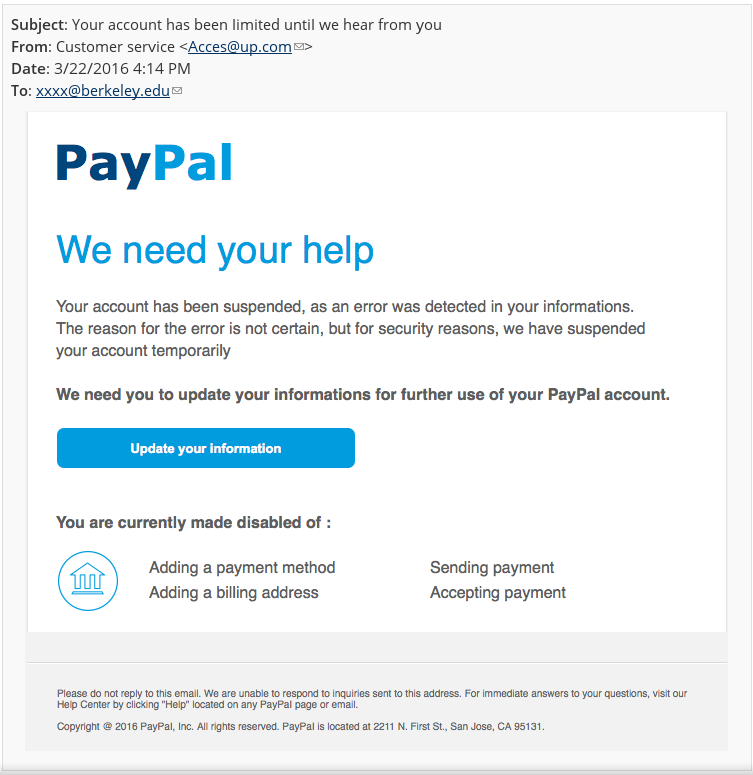
\includegraphics[width=1.0\textwidth]{phishing_example_paypal.png}
    \caption{This figure shows a phishing email disguised to appear to come from Paypal. The link shown in the email leads to a fake login page which allows the attacker to steal user credentials.}
   \label{fig:phishing-example-paypal}
\end{figure}
\begin{figure}[p]
\centering
    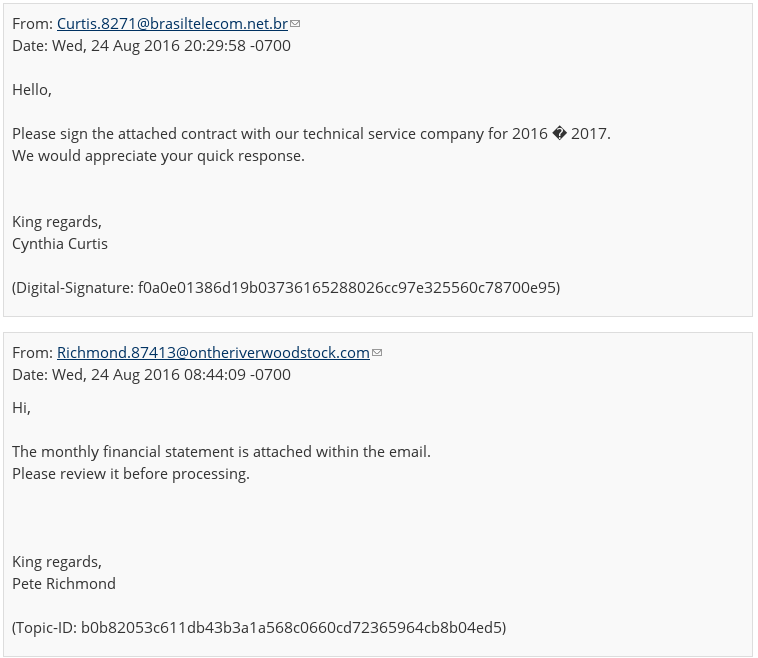
\includegraphics[width=1.0\textwidth]{phishing_example_malware.png}
    \caption{This figure shows a phishing email with an attachment that, when executed, installs a ransomware onto the user's computer.}
   \label{fig:phishing-example-malware}
\end{figure}

Figure \ref{fig:phishing-example-paypal} shows a phishing email \cite{phishing-example-paypal} that appears to originate from Paypal, an online money transaction service. It asks the user to click on a link to update their information. Upon clicking, the user is redirected to a fake Paypal login page intended to steal the user's credentials.

Figure \ref{fig:phishing-example-malware} shows a phishing email \cite{phishing-example-malware} with an attachment that appears to contain the user's monthly financial statement or a service contract. The attachment is a malicious file which, upon execution, encrypts all the files on the computer and shows a ransom message on the screen.

As recent attacks have demonstrated, current systems do not take sufficient measures to protect users from phishing attacks. Such attacks may take place through various methods and are hard to defend against. In most cases, users are either not careful enough, or are unaware of the expectations from genuine sources. Therefore, they miss the cues that tells them that a phishing attack is taking place. This thesis presents the design of \namesecureworkstation/, a workstation to better defend against cyberattacks, specifically phishing attacks.

\section{Approach}

\namesecureworkstation/ is composed of three parts: (i) Qubes OS, a virtualization-based operating system that provides strong isolation guarantees, (ii) a HTTP/HTTPS proxy filter that uses the technique of deep packet inspection \cite{deep-packet-inspection}, (iii) a secure and unambiguous user interface for browsing the web, and (iv) a filtering policy called Site Aggregate Isolation.

The goal of Quboid is to defend against phishing sources, specifically phishing attempts which occur through user-created content such as public forums, instant messaging, emails, etc. We introduce a new filtering policy called Site Aggregate Isolation. The policy dictates that websites with logically unrelated content must not share state and should not be able to communicate with each other. For example, Gmail and Bank of America are different products and should be isolated whereas Facebook Web and Messenger may be allowed to share state. Current systems lack the mechanism to reliably identify which website is being displayed to the user. Phishing attacks take advantage of this to trick the user into trusting the phishing content to be genuine. We believe that the policies introduced in this thesis will help reducing this ambiguity and thus provide stronger guarantees for preventing phishing attacks.

\namesecureworkstation/ implements the Site Aggregate Isolation policy in two places. Firstly, it uses separate browser instances to isolate websites belonging to different site-aggregates, a group of related websites. It uses Qubes OS \cite{qubes-os}, an operating system that uses virtualization for isolation, to run each browser instance in an isolated virtual machine. This ensures that no state can be shared between different site-aggregates. This also ensures that in the event one browser instance gets compromised, the damage is limited to just that virtual machine.
Secondly, traffic from each virtual machine is routed through an intermediate proxy VM. The proxy VM is responsible for filtering requests and enforcing the rest of the Site Aggregate Isolation policy.

For security in user interaction, \namesecureworkstation/ also contains of a secure user interface. The interface consists of a single application window manager restricted to displaying only one browser instance on the screen at anytime. A part of the screen is reserved exclusively for showing the site-aggregate name of the active browser instance. We believe these steps help prevent phishing attacks by reducing the ambiguity of the user interface.

\section{Contributions}

This thesis introduces a set of new policies. These policies allow a safer browsing experience with some loss of usability. The policy design includes the following:

\begin{itemize}
    \item a website identification and isolation mechanism called \textit{Site Aggregate Isolation},
    \item exceptions to this policy to allow websites to refer to external resources and communicate with websites belonging to other site-aggregates, and
    \item guidelines for the interface of the browsing client to reduce the ambiguity regarding the site-aggregate name of the content shown on the screen.
\end{itemize}

This thesis also presents an implementation of these policies in the form of a workstation. The implementation includes the following:

\begin{itemize}
    \item \namesecureworkstation/, a system developed on top of Qubes OS to open browser instances belonging to different site-aggregates in separate virtual machines,
    \item set of HTTP response headers that include additional information such as the site-aggregate name of the website, set of external resources needed, etc., and
    \item a secure user interface with reserved areas for the system and the applications, and a clear display of the site-aggregate name of the currently active browser instance.
\end{itemize}

It is difficult to ensure that no malicious content is encountered by a user while browsing the web. The principal contribution of \namesecureworkstation/ is an increased awareness in the ability of the user to identify malicious content and safely browse the web without any harmful effects.

\paragraph{Limitations:} A major part of our proposed system requires changes in the structure of existing websites. Quboid introduces a number of HTTP header fields in our design. Since these are new header fields, current websites will have to include them in their implementation. Furthermore, a possible misconfiguration by website developers may still leave the users vulnerable to phishing attacks.

\namesecureworkstation/ defends against some but not all forms of phishing attacks. Although the system takes several steps to reduce the possibility of a successful attack, the security of the system still rests in the hands of the user. The interface provides cues to the user when there is a possibility of a phishing attack. If the user is not careful enough to recognize them, they may still fall victim to phishing attacks.

The everyday browsing experience of the user is also changed. Quboid offers strict isolation when browsing the web. This means if users want to download a new software, it will also be run in an isolated virtual machine. The system does not provide an easy way to interact with other software running in different virtual machines.

\section{Outline of thesis}

Chapter~\ref{chap:relatedwork} describes related work regarding creating secure workstations. We analyze the different approaches taken by modern-day systems, ranging from a full-blown operating system to methods like spam filters in email clients. We begin by describing the different ways phishing attacks operate, followed by analyzing each system to see where they fail in defending against such attacks.

Chapter~\ref{chap:goals} describes the goals of this thesis. We list properties a secure workstation must have to prevent phishing attacks. Additionally, we give examples of phishing attacks to justify the importance of these properties. We emphasize a secure workstation's ability to block malicious content, present an unambiguous user interface, and contain damage in the event of a breach.

Chapter~\ref{chap:design} describes the design of the workstation proposed in this thesis. We describe in detail new policies targeted at attacks originating from user-created content. We also describe ways to implement these policies in a proxy filter using the technique of deep packet inspection.

Chapter~\ref{chap:implementation} gives the implementation details of \namesecureworkstation/. We describe the different subsystems used and the pros and cons of some alternate implementations of these subsystems.

Chapter~\ref{chap:analysis} analyzes the effectiveness of the system as a whole in defending against recent real-world phishing attacks and various fictional phishing scenarios. Of course, our system does not defend against all forms of foreseeable attacks, however, it is able to defend against a majority of attacks that current systems do not.

Chapter~\ref{chap:conclusion} concludes this thesis with a summary of \namesecureworkstation/. A majority of cyberattacks start off with a phishing attack on an unsuspecting user. The secure workstation developed focuses on the heart of the methods used in these cyberattacks. Our hope is that with this workstation, users are able to browse the internet without worrying about downloading unsolicited software from unknown websites or having their details unsuspectingly stolen during day-to-day browsing.
\chapter{Related Work} \label{chap:relatedwork}

This chapter describes existing systems used to create secure workstations. We provide a brief summary of each of the following systems and analyze its limitations.

\paragraph{Qubes OS:} Qubes OS is an operating system which uses virtualization to provide isolation. It provides features such as the ability to create tiered VMs based on security levels, firewall policies to restrict network traffic in respective tiers, and a secure user interface implementation. Quboid uses Qubes OS as its base to preset a secure workstation.

\paragraph{Bromium:} Bromium is a similar system to Qubes OS which uses a technology called micro-virtualization to provide similar isolation guarantees while retaining the performance benefits of traditional OS processes. The idea of running each application in a separate virtual machine is used in the design of Quboid.

\paragraph{Google Chrome Browser:} The Google Chrome Browser uses isolation techniques to execute tabs in a sandbox. This largely prevents attacks that take advantage of browser exploits. Quboid has a similar goal to Chrome Browser - to provide users the ability to browse the web safely.

\paragraph{Spam Filters:} Since most cyberattacks begin with a phishing email, we analyze the spam-filtering systems used by Gmail, a popular email provider. We analyze the effectiveness of the parameters used by the Gmail filters and its limitations.

\paragraph{EROS Trusted Window System (EWS):} The user interface is another system which phishing attacks take advantage of. EWS is a system which uses the concept of trusted path for user interaction to provide a trusted window system.

\section{Qubes OS} \label{section-qubes-os}

Qubes OS is a security oriented operating system based on Xen hypervisor \cite{xen}. It uses virtualization to provide isolation among applications running in different security levels. Users have the ability to create virtual machines and designate them with different security levels for use with different applications. For example, banking and credit card applications can reside in a trusted VM whereas general everyday browsing can occur in an untrusted VM. The Qubes OS interface is a GUI running in Xen's dom0, the built-in trusted VM which is allowed to perform management operations on the hypervisor. Qubes OS provides several features to ensure that dom0 is never compromised even if one of the virtual machines gets compromised.

The following subsections describe the isolation guarantees provided through virtualization, firewall policies for the VMs and the Qubes user interface:

\subsection{Isolation using Virtualization}

The virtual machines in Qubes OS run complete operating systems. However, they all share the same root filesystem which is read-only. Any modifications done by the VMs to the root filesystem are performed in-memory and are rolled back when the VM is shut down. Additionally, each VM also has a personalized home filesystem which stores persistent data.

Having such a strict isolation between different VMs provides better security but also decreases usability. Qubes OS has the following features to overcome this limitation:

\paragraph{Clipboard Sharing} Qubes OS lets VMs copy and paste data to and from their own clipboards through the use of shared memory between VMs. The dom0 is not involved in the data exchange which reduces the attack surface.

\paragraph{Disposable VMs} A user may want to run an application just once in a separate isolated VM. In a normal workflow, the user will have to create a new VM with an operating system, run the application in it, and then delete the VM. To simplify this workflow, Qubes OS has a feature called Disposable VMs. A disposable VM runs like a normal VM but has an ephemeral hard disk. It can be booted up within seconds to run an application and then destroyed. It is based on an existing template so the user does not have to reinstall the operating system every time a new disposable VM is created.

\subsection{Firewall Policies}

Qubes OS implements strict network isolation. No inter-VM communication is possible unless the user explicitly modifies the configuration. Network traffic from each VM is routed through an intermediate VM called the FirewallVM. The FirewallVM runs a traditional port-based firewall called {\tt iptables}. Users can change the firewall policies through the VM management interface. However, these policies are limited to allowing or denying traffic to and from a specific IP address and/or port.

The management VM, dom0, is completely isolated and has no network access. This ensures any outside attacks are not able to target and compromise dom0. If dom0 requires network access, for example when performing an update, the necessary files are downloaded into a separate VM, checked for integrity and then copied over to dom0 through the use of shared memory.

\subsection{User Interface}

The user interface is an important aspect to focus on to combat phishing attacks. Most phishing attacks pretend to be a trusted website in order to trick the user into entering their credentials and other sensitive information. Qubes OS makes sure that all applications running in different security levels appear visually separate from each other through the use of window border colors. For example, the trusted VM can have a green border color whereas the untrusted VM can have a red border color. The users must ensure that they only enter their information in the trusted VM when they see a green border color around the application. The user is also allowed to rename the VMs which provides an additional method to verify that they are entering their information in the correct VM. Figure~\ref{fig:qubes-screenshot} shows a screenshot of the Qubes OS user interface.

\afterpage{\clearpage
\begin{figure}[p]
\centering
    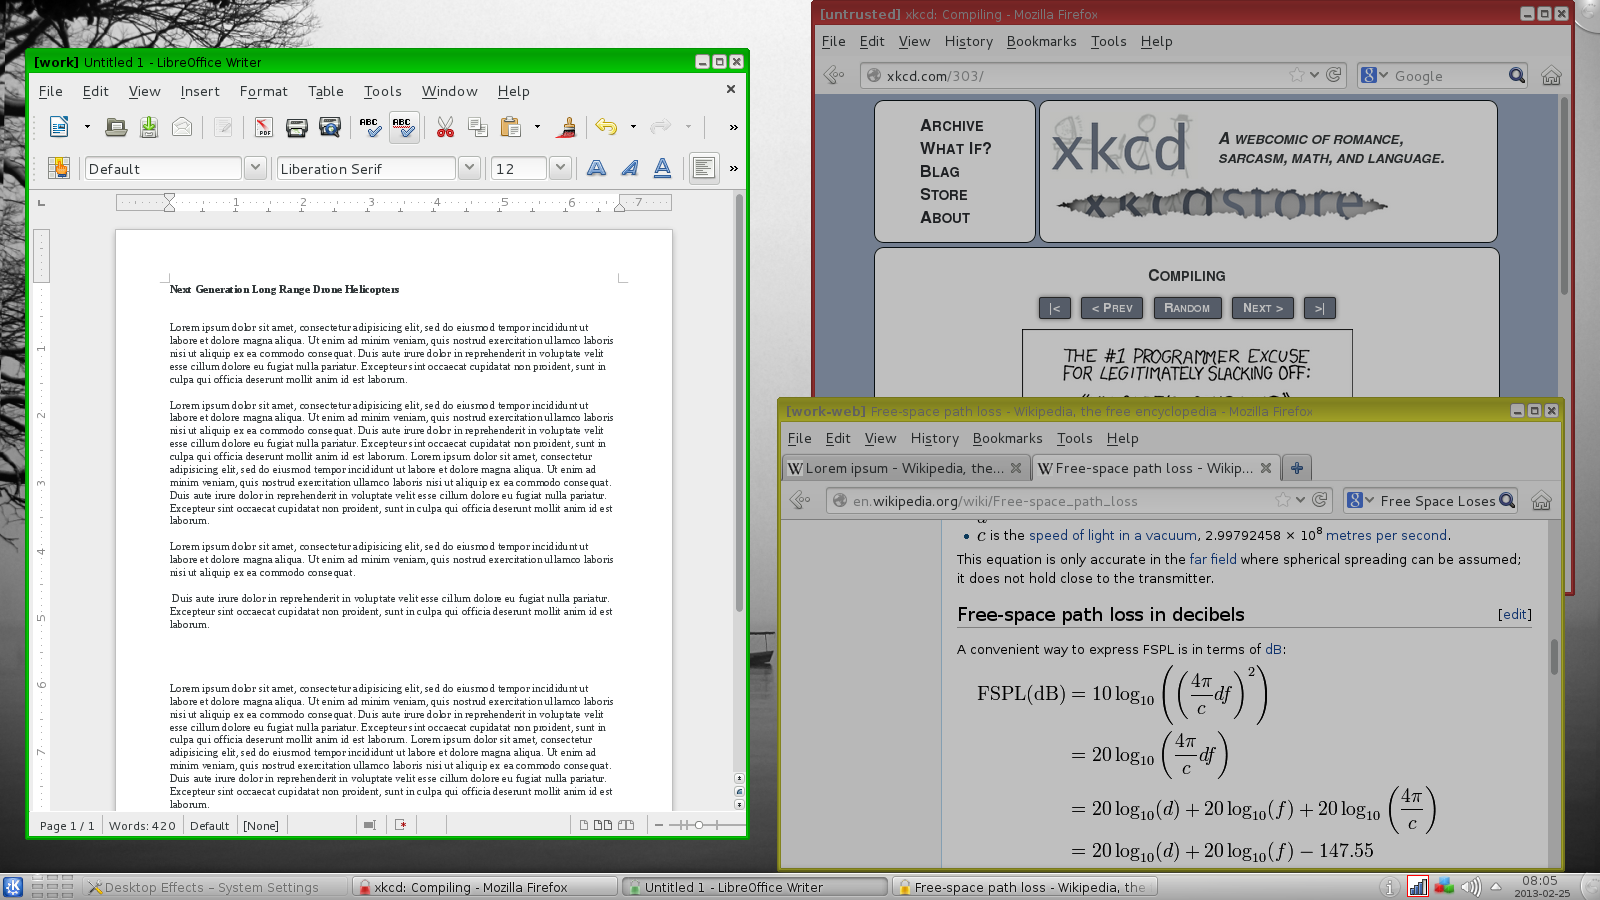
\includegraphics[width=1.0\textwidth]{qubes-screenshot.png}
    \caption{This screenshot shows the user interface of Qubes OS. Each of the applications is running in a separate virtual machine. The user has labelled the virtual machines as [work], [work-web] and [untrusted], and have given appropriate border colors to visually differentiate the virtual machines.}
   \label{fig:qubes-screenshot}
\end{figure}
\clearpage
}

\subsection{Limitations}

Although Qubes OS provides strong security guarantees, it has its limitations for defending against phishing attacks.

\paragraph{No support for advanced firewall rules:} The firewall is only able to filter based on IP and port. Advanced filters based on hostnames are unavailable. This is specially important because a user may want to designate a VM as their bank VM and have firewall rules prohibiting any traffic except to their bank. If the bank's website changes IP addresses, for example via a load balancer, an IP and port based firewall proves insufficient. The Site Aggregate Isolation policy described in this thesis requires the use of advanced filter rules.

\paragraph{Ambiguity in the user interface:} The border color and custom naming strategy is not enough to defend against some phishing attacks. Qubes OS uses a stacking window manager. It can have multiple resizable windows which can be stacked on top of each other. It is possible for an untrusted VM window to pretend to contain a trusted VM inside its bounds and can trick the user into entering their credentials into the untrusted VM.

\section{Bromium}

Bromium \cite{bromium} is a virtualization-based system similar to Qubes OS in several aspects. It uses virtualization to run applications in separate virtual machines, similar to Qubes OS. One major difference is instead of running a full operating system in a VM, it uses a technology called micro-virtualization. Micro-VMs are lightweight processes which share a lot of resources with the hypervisor while still retaining the isolation guarantees obtained by running full virtual machines. This allows users to quickly launch applications in new virtual machines without going through an OS boot cycle.

Another feature provided by Bromium is the ability to preform post-exploitation analysis. If the system determines that a possible attack is underway, it notifies the user and allows the user to perform analysis on the attack. While attacks are still possible, the damage is contained to the virtual machine where the infected application resides. It is unable to compromise the rest of the system.

The ability to run application in separate VMs is specially effective against ransomware attacks. In such types of attacks, the malicious software encrypts the whole hard drive, sends the decryption keys to the attackers, and deletes those keys from the local system. The only way to recover the data then is to pay the attackers a sum of money in order to retrieve the decryption keys. Figure~\ref{fig:wannacry} shows a screenshot of the prompt shown after the WannaCry ransomware has finished the encryption. This was a recent ransomware attack which compromised several U.K. hospitals.

\afterpage{\clearpage
\begin{figure}[p]
\centering
    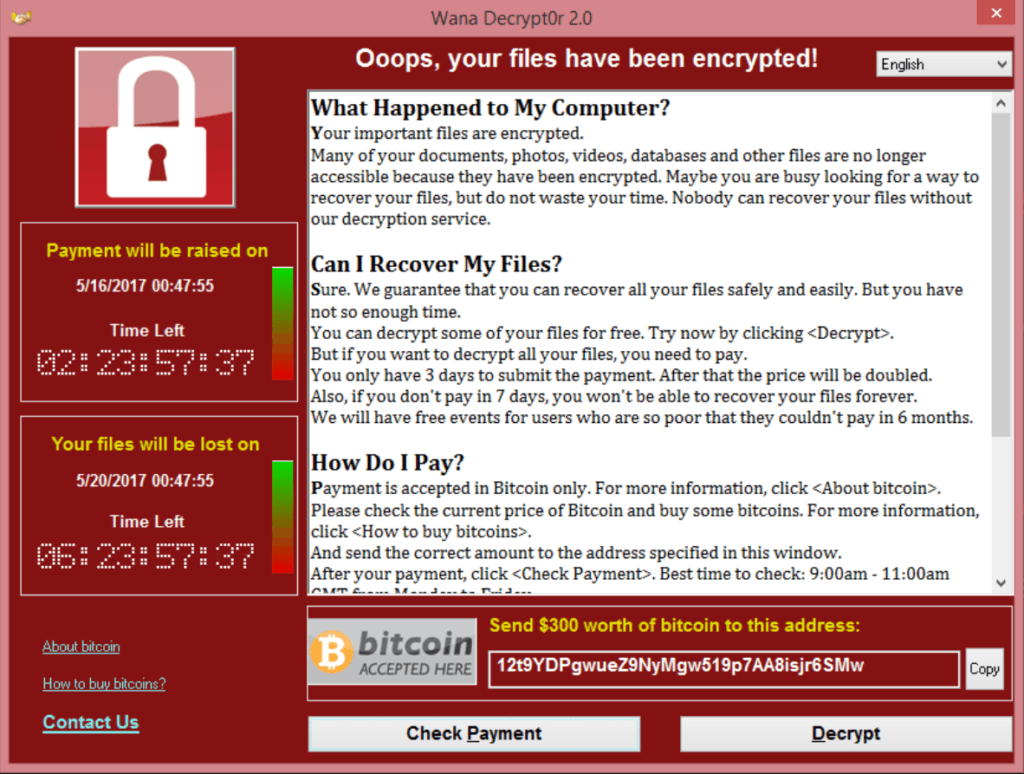
\includegraphics[width=1.0\textwidth]{wannacry.png}
    \caption{This screenshot shows the prompt shown after the WannaCry ransomware has finished encryption of the whole hard disk. The attack uses a bug in the OS to compromise the whole system. It then encrypts the hard disk, sends the decryption keys to the attackers and then deletes those keys from the local system. The only way to recover the keys is by paying the attacker \$300 via Bitcoin and hoping to re-obtain the decryption keys.}
   \label{fig:wannacry}
\end{figure}
\clearpage}

If a ransomware was to attack a system running Bromium, it will only have access to the hard disk associated with the virtual machine where the application is running. Once the application is closed, the virtual machine is shutdown destroying all traces of the attack. 

Qubes OS also shares similar advantages, however, it is possible to have multiple applications installed in the same virtual machine. The ransomware attack could still
encrypt the contents of the other applications. Bromium provides a stronger security guarantee by executing each application in its own virtual machine.

\subsection{Limitations}

Although Bromium defends against phishing attacks that lead to downloading malicious software, it does not defend against phishing attacks that are designed to steal user information. Bromium provides no defense against attacks that are designed to trick the user into entering sensitive information and steal their details, for example, a website can still display a fake login form and Bromium will not give any indication that something is wrong.

\section{Google Chrome Browser}

The Google Chrome Browser is a popular modern-day browser. It has been the leader of the browser market share for more than a year, surpassing Microsoft Internet Explorer in March 2016 in the desktop browser market share \cite{marketsharereport}. It provides a simple user interface and several features to increase the usability and security of the browser. However, the highlighting feature of Chrome is its sandbox.

The Chrome sandbox \cite{chromesandbox} is a mechanism to provide guarantees on what a piece of code can and cannot do. The rendering engine of each tab is run in a sandbox. The sandbox leverages existing operating system mechanisms to restrict the privileges the code has. It forbids access to the file system, display, clipboard, operating system hooks, etc. The rendering engine draws onto an off-screen buffer which the browser then displays to the user.

The threat model for the sandbox operates under the assumption that the code executing is malicious and the sandbox has been compromised. Thus, a lot of features are focused on making sure the code cannot take advantage of browser bugs to compromise the system.

\namesecureworkstation/ uses similar ideas as Google Chrome, for example, executing code from different websites in isolation from each other. The virtual machine in \namesecureworkstation/ serves the same purpose as the sandbox serves in Chrome. Virtualization is a step forward in providing isolation in additional contexts, such as the ability to execute malicious executable file in a contained environment.

\subsection{Limitations}

The Chrome sandbox contains any code running within a tab in a sandbox. However, it does not prevent any downloaded code to execute in an isolated environment. If the user downloads a malicious file, it will still be able to compromise the entire system.

Additionally, Chrome does not have mechanisms to prevent phishing attacks. Similar to most other browsers, it warns the user about inconsistencies in the browser SSL/TLS certificates. It also maintains a blacklist of malicious websites and warns the user when navigating to such websites. However, any website not in the blacklist or with valid certificates can still be able to trick the user into compromising their credentials.

\section{Spam Filters}

A lot of phishing attacks use emails to spread. A recent attack \cite{google-docs-phishing} started with users clicking on a phishing email which pretended to contain a link to a shared document on Google Drive. The attackers were then able to obtain the user's Gmail authentication token which was used to automatically forward the email to everyone on the user's contacts list. Fortunately, most of the email providers implement some sort of spam filtering before the email reaches the user's inbox to prevent such sort of attacks.

For example, Gmail uses the following list \cite{gmail-spam-filter-list} to determine when emails should be automatically marked as spam. We only list the parameters which are relevant for defending against phishing attacks:

\paragraph{Spoofed email addresses:} If the sender's email address is very similar to a known email address, for example {\tt contact@company.org} and {\tt c0ntact@company.org}, users may mistake the latter to also be a legitimate source. Gmail recognizes such spoofs and automatically marks them as spam.

\paragraph{Known phishing scams:} Gmail lets users mark emails as phishing. If enough users mark similar looking emails as phishing, it is an indication that any such future emails should be automatically marked as spam. However, this strategy fails if the phishing scam is new and not enough feedback has been gathered from user reports.

\paragraph{Messages from unconfirmed sender:} If Gmail is unable to verify that the email was sent from the source it claimed to be sent from, it is marked as spam. This strategy is helpful when attackers try to send emails with legitimate source email address from unauthorized email servers, for example, public SMTP servers.

\subsection{Limitations}

Although these strategies are helpful against most phishing attacks, some phishing email may still end up in user's inbox. Emails that originate from legitimate email addresses, or attacks which are fairly new and haven't been flagged yet can bypass these mechanisms.

\section{EROS Trusted Window System}

The EROS Window System (EWS) \cite{eros} is a window system which provides strict access controls to the user and claims to not introduce any new covert channels in the display system. It is a minimal implementation of a secure window system and is under 4,500 lines of code. The system provides isolation between applications and allows no communication between them unless the user has specifically authorized so.

The system makes sure that any communication between application should only be allowed if it can be traced by back to an authorizing user action. This system also addresses some part of user interface security. In particular, it provides a small code footprint which is easy to very for security bugs. It addresses partially the issue of user interface ambiguity by using different brightness for active and inactive windows.

An important property that this system provides is the principle of isolation and restricted communication. Client sessions operate in isolation of each other, no session can affect or observe state from other sessions. Additionally, the display server restricts the kind of communication that can place between processes. The design of \namesecureworkstation/ applies the idea of isolation and restricted communication to different websites i.e. different websites must not share state and there must be restricted communication between them.

\subsection{Limitations}

EWS is a not complete secure workstation solution. It addresses the issue of security between different processes on the system. However, security while web browsing requires a completely different solution. Several forms of phishing attacks don't rely on faking windows and window actions. We can however take inspiration from the ideas of EWS such as isolation and restricted communication to design a secure workstation.

\chapter{Goals} \label{chap:goals}

Systems such as Qubes OS, Bromium and Chrome are successful in preventing attacks that exploit software bugs. However, their security guarantees are insufficient to prevent phishing attacks. In this chapter, we list the properties of an ideal secure workstation. We also list attack scenarios that the workstation would be able to prevent.

\paragraph{Blocking malicious content:} The primary property of a secure workstation is the ability to block malicious content. Malicious content can be accessed by users in various ways: the website the user is visiting may have been compromised, malicious content could have been posted by an attacker on a public forum, or users may explicitly navigate to a malicious website. The system must take steps to identify such content and block it from being displayed.

\paragraph{Unambiguous User Interface:} A lot of phishing attacks operate by displaying a fake login page to the user. A secure workstation must ensure that the user can only enter sensitive information in genuine websites, and have mechanisms to defend against fake websites.

\paragraph{Damage Containment:} Even after taking several precautions, some damage is inevitable. We cannot foresee all sorts of future attacks that may come up. The secure workstation must ensure that in the unlikely event of a malicious software being able to execute, the damage caused is contained. The risk of leaking sensitive information in such events must be minimized.

The rest of this chapter focuses on case studies to make the goals of the secure workstation more concrete.

\section{Blocking Malicious Content}

Several phishing attacks operate by including malicious content in places which appear to come from legitimate sources. This content can include malicious software, fake login pages, etc. Below we list two phishing scenarios which highlight ways these attacks operate.

\paragraph{Fake Gmail Attachment Scam: }
The first case we look at is a phishing email scam \cite{fake-attachment-scam} which uses fake attachments in order to lure the users into clicking on it. The email has an image of what looks like a Gmail attachment but in-fact is a link to an external page. Figure~\ref{fig:fake-attachment} shows how the email appears to the user.

\begin{figure}[p]
\centering
    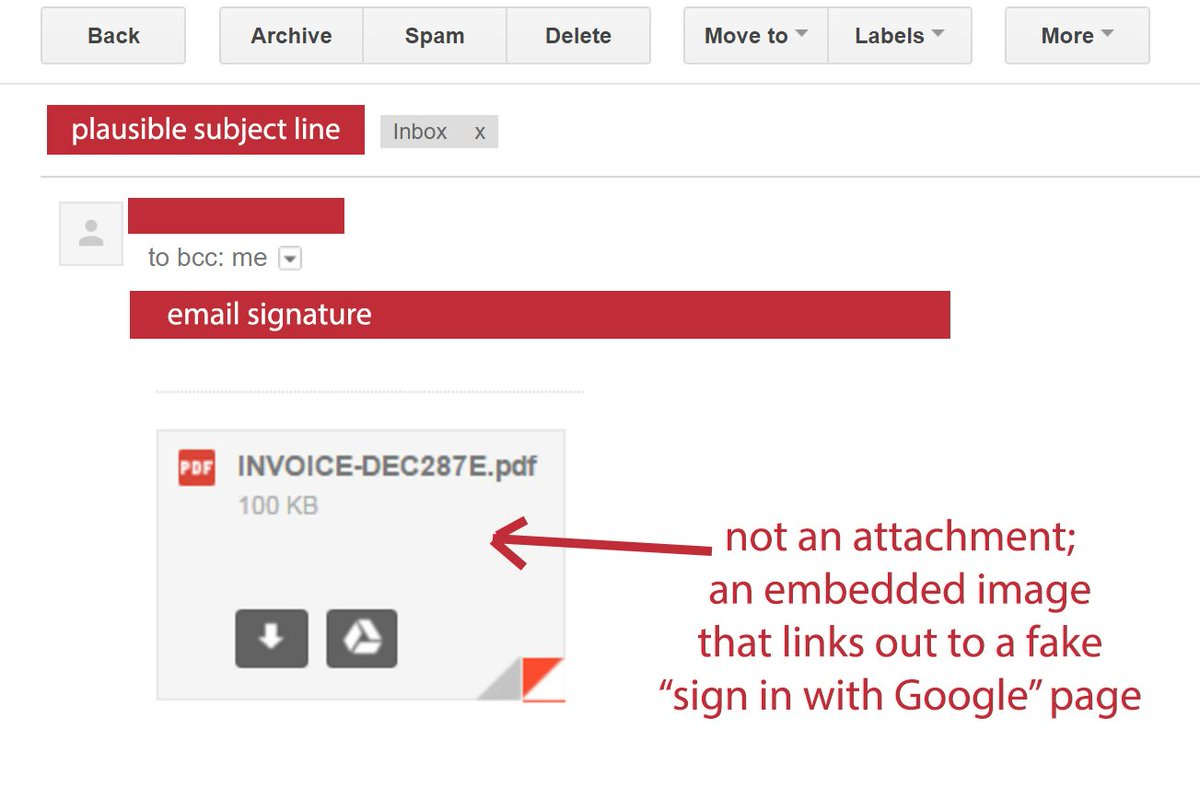
\includegraphics[width=1.0\textwidth]{tomscott-gmail-phishing.jpg}
    \caption{The email in this figure has an image which appears to be an attachment but in-fact is a link to an external page which displays a login page.}
   \label{fig:fake-attachment}
\end{figure}

Figure \ref{fig:fake-attachment-login} shows the page displayed when the user clicks on the fake attachment link. This page shows several other features that are common among phishing attacks such as a deceptive URL, similar looking Google login page, missing SSL/TLS certificates which would identify this page as belonging to Google, etc. The attackers can steal the credentials that the users enters on this page.

\begin{figure}[p]
\centering
    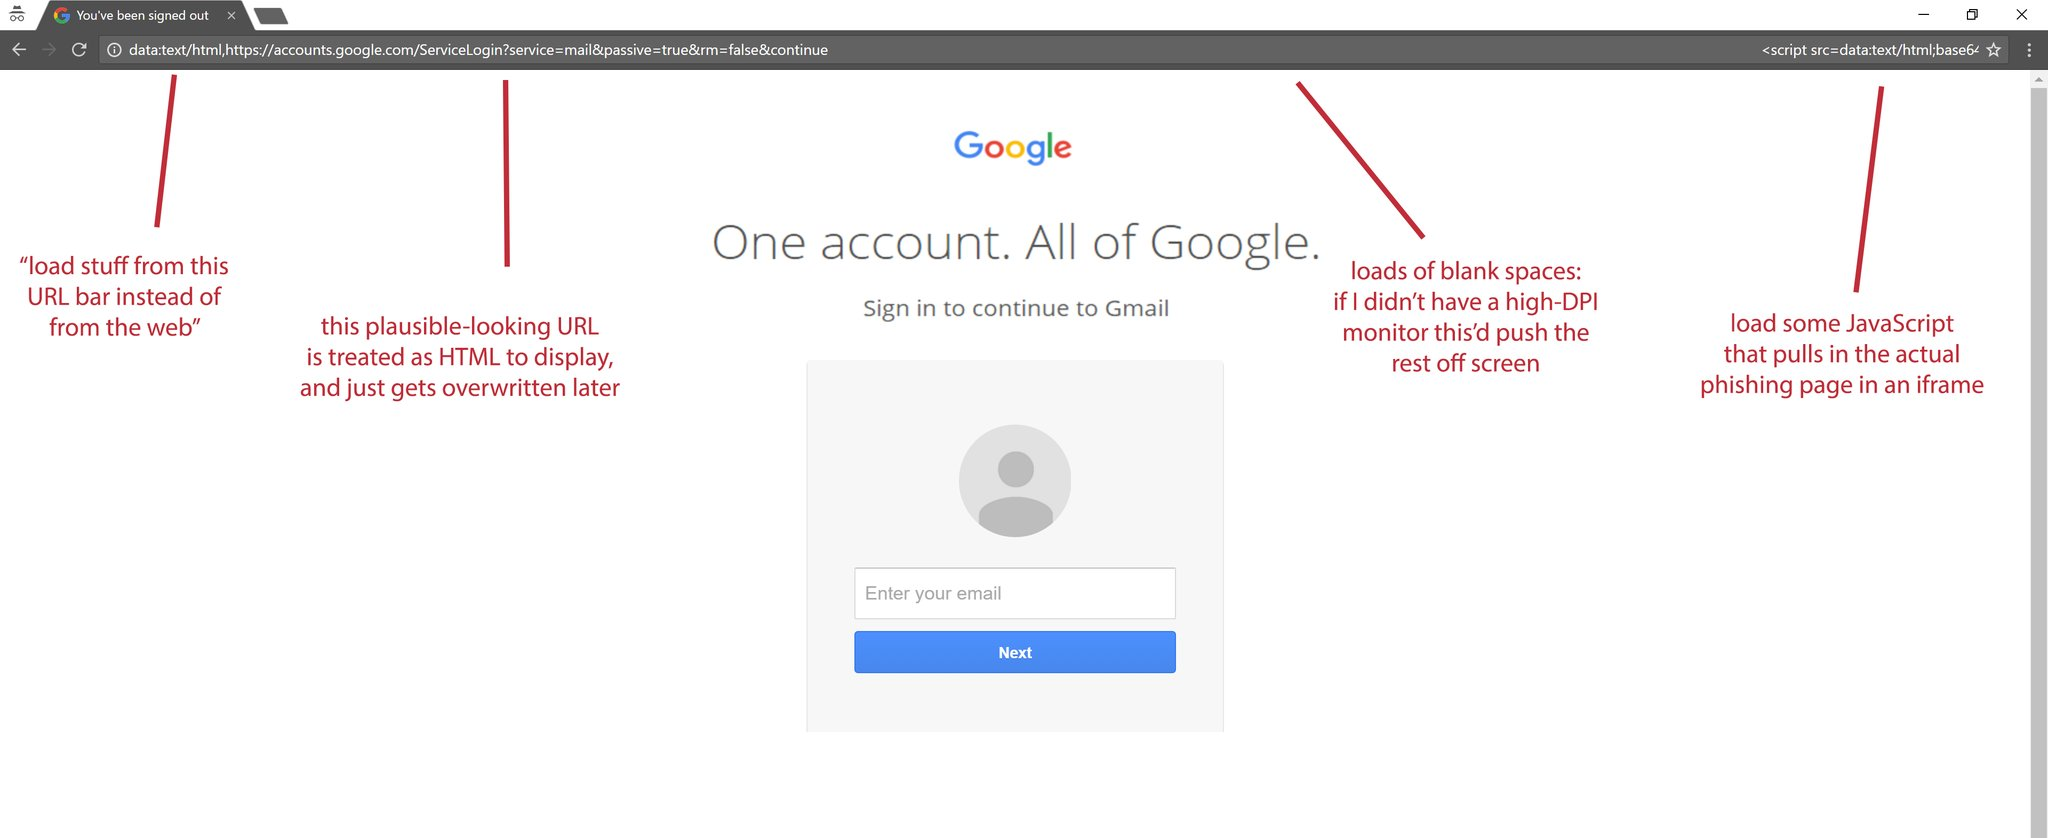
\includegraphics[width=1.0\textwidth]{tomscott-gmail-login.jpg}
    \caption{Clicking on the fake attachment leads to this fake login page.}
   \label{fig:fake-attachment-login}
\end{figure}

There were other ways this attack could have worked. The attachment link could have led to an external URL which would have download a malicious software into the user's computer. A secure workstation must be able to defend against such attacks. It should include mechanisms to avoid displaying such links, stopping the download of malicious software or prevent users from getting tricked into entering credentials into fake login pages.

\paragraph{Malvertising:} The second case we analyze is of malvertising \cite{malvertising}, malicious advertisements displayed on legitimate websites. Consider a recent attack \cite{malvertisement-nytimes} that used malvertisements on major news outlets like New York Times, BBC, etc. Attackers were able to inject malicious software in legitimate online ad networks. When users visited the website, it would redirect them to the attackers website which would target security holes in software such as Microsoft Silverlight and Adobe Flash. If the compromise was successful, a ransomware would get installed and encrypt the users files.

A major factor responsible for the success of this attack was that the news outlets trusted the external ad services into displaying anything in their webpages. There was no protection that in the unlikely event these services get compromised, the outlet websites do not get affected. A secure workstation must be able to defend against such attacks by including mechanisms to restrict the trust placed in externally linked content.

In summary, for a workstation to be secure against malicious content, it should have the following properties:

\begin{itemize}
    \item Mechanisms to \textbf{block malicious content} to be displayed in the first place,
    \item Methods to identify and \textbf{differentiate genuine content from malicious content}, and
    \item \textbf{Fallback mechanisms} in case of a compromise in a subsystem.
\end{itemize}

\section{Unambiguous User Interface}

Exploiting the user interface is another mechanism through which phishing attacks operate. The main goal of phishing attacks is to trick the user into believing the phishing content to be genuine. We analyze some of these ways below.

\paragraph{Faking other websites:} Some phishing websites operate by appearing to be a duplicate of a genuine website. Some may even have similar looking domains names. These websites usually present a login form to the user where the user is tricked into entering their credentials. Upon submitting the login form, the attackers can steal their credentials and optionally redirect the user to the genuine login form. The user is lead to believe they have mistakenly typed their password incorrectly and they are none the wiser.

As an example, consider the case of the usage of Punycode in browsers. As the world is adopting Unicode, it is possible to use any Unicode characters in browsers. To encode non-ASCII characters, browsers use a encoding called Punycode. A recent vulnerability \cite{punycode-attack} discovered takes advantage of the encoding of similar looking characters to display websites whose domain name appears visually indistinguishable from real domain names. Further, it is possible to also obtain free SSL/TLS certificates for the fake domain names. The only way for the user to tell the difference between a real and a fake website is then to explicitly check the certificate. For example, domains names can use both a Unicode Cyrillic small letter ``a" or a Latin small letter ``a". Both look visually indistinguishable. We can encode the domain {\tt apple.com} using alternative characters in Punycode as {\tt xn--80ak6aa92e.com}. When shown in browser, both domains appear identically as {\tt apple.com}. Figure~\ref{fig:punycode-apple} shows how both domains appear in the browser.

\begin{figure}[p]
\centering
    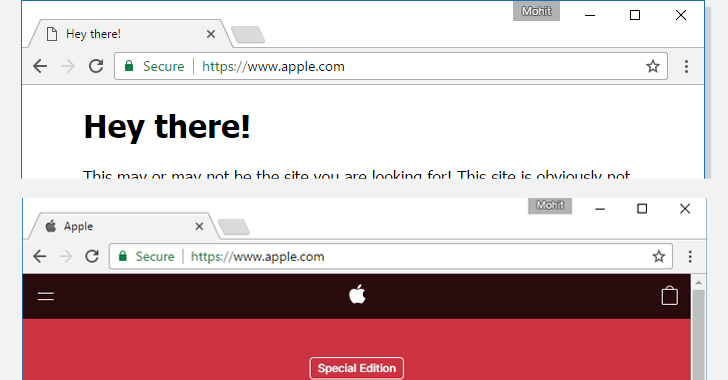
\includegraphics[width=1.0\textwidth]{punycode-apple}
    \caption{Both domain names are similar except their use of the small letter ``a". One uses a Unicode Cyrillic ``a" whereas the other uses a Latin ``a".}
   \label{fig:punycode-apple}
\end{figure}

A secure workstation must be able to mitigate such attacks by including mechanisms to verify that the website the user is visiting is the website the user intended to visit.

\paragraph{Faking system prompts:} Another common way that phishing attacks operate is by showing fake system prompts. One popular attack works by showing a fake prompt to the user displaying that the user's computer is infected and asking them to click on a link to download an antivirus software. The link in reality downloads a malicious software to compromise the user's computer.

A secure workstation must have mechanisms to let the user distinguish between content displayed by the system and content displayed by the website. It must \textbf{provide ways to distinguish fake and genuine content}.

\section{Damage Containment}

Even after taking all the precautions, it is still very hard to stop all kinds of attacks. Thus it is important to plan how a secure workstation would handle a compromised system. The primary principle to be followed in case of a security breach should be to contain the damage as much as possible. For example, if a webpage gets compromised no other webpages should be affected, or if a browser instance gets compromised no other browser instances should be affected.

We will analyze the case of ransomware attacks to understand why damage containment is important even after the system gets compromised. A ransomware software needs to be first executed on a system to take effect. It can be downloaded by following malicious links that download unsolicited software on the computer, or by opening malicious attachment in an email client. Once a ransomware software executes, it starts encrypting all of the content of the hard disk in order to leave files inaccessible. The ransomware then sends the decryption key to the attacker and deletes the key from the system. After that, it displays a prompt notifying the user that their files have been encrypted and demands a payment for the decryption key to be made available again in order to decrypt the files. There is usually no defense against a ransomware attack after the encryption has taken place other than paying the ransom and hoping to recover the files.

The principle of damage containment can play an important role when faced with a ransomware attack. A secure workstation must have mechanisms in order to \textbf{limit the damage that such malicious software can do}. For example, in case of ransomwares, the system can provide isolation and restrict filesystem access. This will restrict the damage the ransomware can do.
\chapter{Design} \label{chap:design}

This chapter presents the design of a workstation to reduce impact of phishing attacks. Phishing attacks usually operate by misleading users into trusting malicious content as being genuine. The design includes several policies to be enforced by the browsing client.

\paragraph{Site Aggregate Isolation:} Modern internet applications consist of content from different sources: user-generated content, external APIs, etc. This makes it difficult to identify the source of the content a users sees. Phishing attacks take advantage of this by displaying content that appears to be created by a genuine source. We present a new policy called Site Aggregate Isolation to defend against such attacks. The policy dictates that content from different sources (or \textit{site-aggregates}) must be explicitly displayed in isolated environments.

\paragraph{Cross Site-Aggregate Resources:} Since applications need to display content from different site-aggregates, we describe exceptions to the Site Aggregate Isolation policy for resources to be included from other site-aggregates in a safe way.

\paragraph{External Resource Referrer:} Some attacks operate by stealing information from external websites, for example, by stealing information from internal APIs belonging to third-party websites. We introduce a policy to defend against such unauthorized cross site-aggregate requests.

\paragraph{Exit Destinations:} Modern applications also rely on communication among one another. Phishing attacks take advantage of this by being able to steal information and submitting it to the attacker's server. We present a policy to defend against unauthorized communication between websites.

\paragraph{HTTP Response Headers:} The policies presented in this chapter requires additional information from websites. Websites currently do not provide information about their site-aggregate name, external resources they require, or external URLs they may communicate with. To extract this information from the websites, we introduce four new HTTP response headers: \texttt{Site-Aggregate},  \texttt{Site-Aggregate-Pattern}, \texttt{Cross-Site-Aggregate-Resource-Pattern}, and \texttt{Exit-Pattern}.

\paragraph{DNSSEC and SSL/TLS Certificates:} A popular way phishing attacks operate is by DNS spoofing or DNS cache poisoning. We present policies to prevent against these attacks.

\paragraph{User Interface:} In addition to securing the web browsing backend, we present the design of a secure user interface. Phishing attacks trick the user by taking advantage of the ambiguity of the user interface. We discuss the limitations of the current user interfaces that use stacking window managers. We also present a clear and unambiguous user interface by introducing a single-application window manager inspired by smartphones.

\section{Site Aggregate Isolation} \label{same_origin_isolation}

While browsing, one of the primary concerns of the user is to ensure that the content they see is genuine. One way to approach this would be to forbid all content that was not created by the owner of the website the user intended to visit. However, such a strict policy would be impractical. Modern internet applications rely heavily on content from several sources, for example, user-generated content, external APIs, etc. Additionally, applications such as social networking websites and email are based around user created content. On the other hand, allowing all content, which is what current browsers do, is also not ideal as it is the main reason behind deceptive content being displayed to the user.

A more flexible policy is needed which still preserves the interactivity of websites allowing them to feature user created content, but also making it clear to the user that certain parts of the website are not created by the website owner and making it visually explicit when the user navigates to a content that was not created by the original website that the user visited.

In the design of a secure workstation, we enforce a policy called Site Aggregate Isolation. An \textit{site-aggregate} is defined as a website or a group of website that coherently form a single unit. For example, Bank of America and Reddit are part of different site-aggregates. The decision to come up with this group is up to the website developers. For example, Google may designate Gmail, Search, News, YouTube, etc. as different site-aggregates. The policy states that web applications belonging to different site-aggregates must be completely isolated from each other, both on the backend side and the user interface side. They must not be able to communicate or transfer data with each other unless both websites explicitly agree otherwise. Additionally, web applications belonging to different site-aggregates must be visually separate and display identifying information about the site-aggregate name at all times.

\section{Cross Site-Aggregate Resources}

Site Aggregate Isolation policy can be too strict for the scenario of websites requesting resources from another website. This is commonly seen for Content Delivery Network (CDN) websites where a popular resource such as a Javascript library is hosted by a mass distribution CDN service and third-party websites can then link back to the CDN and request the external resource. This provides several advantages such as the ability cache common libraries for different websites and faster response times for the resources hosted on the CDN. These external resources however must not be considered as being on the same site-aggregate as a third-party website as they are not served by that website itself.

A policy exception needs to be defined for such resources. The cross site-aggregate resource exception to the policy states that if a website requests resources from an external website not in the same site-aggregate, it must:
\begin{itemize}
    \item provide information such as the cryptographic checksums of the resource so that the browser can verify the integrity of the external resource, and
    \item explicitly enlist the address of the resource in a separate cross site-aggregate resource list.
    \item provide a signature for the cross site-aggregate resource list for the browser to verify that the list has not been tampered with
\end{itemize}
%This is because this can lead to a transitive effect where two websites A and B initially on different origins may be mistakenly considered to be on the same origin since they both list the shared resource on the CDN to be their own respective origin.

\section{External Resource Referrer}

The policy and its exception discussed previously provide safety against a website requesting and displaying resources that the website owner didn't intend to include. However, it doesn't prevent third-party websites from defending against unauthorized requests. For example, Site A may try to access content from Site B however Site B may not want to provide the content to Site A, because that content is internal to Site B.

We implement an external resource referrer policy on all cross site-aggregate resource requests. The policy requires all requests to contain the site-aggregate of the website requesting the resource. Web servers must verify the referrer of all incoming requests and deny serving any requests that are unauthorized for that referrer.

\section{Exit Destinations}

Some phishing websites may still be able to embed themselves into another website. For example, they may be able to inject a HTML form into your social networking feed. They may try to trick the user into entering their password in a fake login form. When the user clicks on the button, they may be redirected to an external page belonging to the attacker where the information may be posted. such attacks may be prevented by restricting the possible exit destinations that a web page is allowed to send information to.

To isolate different site-aggregates and preventing them from sending information to each other, no form data must be allowed to be sent to an external site-aggregate either via a GET or a POST request. However, such a strict policy will again not be able to support modern web applications which may want to submit data elsewhere. To support this, the website must explicitly list all exit URLs in an exit destination list. The website must also provide a signature for this list. The browser must verify the signature and only allow information to be posted if the external URL matches one of the URLs in the exit destination list.

\section{HTTP Response Headers}

The policies introduced in the previous sections require additional information from websites such as their site-aggregate names, list of external resources, etc. We use HTTP response headers to extract this information. In this section, we introduce new HTTP response headers that websites must include to support the system.

\subsection{\texttt{Site-Aggregate-Name}}

Every page must have the {\tt Site-Aggregate-Name} header field which contains the name of the site-aggregate that page belongs to. For example all webpages from {\tt facebook.com} and {\tt fb.com} may have the value of the {\tt Site-Aggregate-Name} header field to be {\tt facebook.com}, since both the domains names are used by Facebook and are part of a single unit. It must be ensured that these names are web-requestable URLs. This is used in verification of the site-aggregate name as explained in future sections.

\subsection{\texttt{Site-Aggregate-Pattern}}

The {\tt Site-Aggregate-Pattern} header field is included in the HTTP response of every web page. This field must include the URL patterns in the form of regular expressions for all the URLs that are considered part of the same site-aggregate as the requested web page. There may be multiple {\tt Site-Aggregate-Pattern} headers in the response which may list additional URLs to be considered part of the same site-aggregate. The filter considers the union of all the site-aggregate patterns to decide if a requested web page is in the same site-aggregate or not.

For example, responses from Gmail may include the following {\tt Site-Aggregate-Pattern} header fields:

\begin{verbatim}
Site-Aggregate-Pattern: https:\/\/mail.google.com\/.*
Site-Aggregate-Pattern: https?:\/\/(www\.)?gmail.com\/.*
Site-Aggregate-Pattern: https:\/\/accounts\.google\.com\/signin\/gmail\/.*
\end{verbatim}

Since multiple instances of the header field are converted to a union, these pattern match any webpages which begin with {\tt gmail.com} or {\tt mail.google.com} domains or are the sign-in pages at {\tt accounts.google.com/signin/gmail}. This ensures that even if any malicious content shows up within these pages, it won't be able to redirect the user to fake login pages outside the Gmail's list of allowed URL's.

\subsection{\texttt{Cross-Site-Aggregate-Resource-Pattern}}

Most webpages include resources from external sources. These may include Javascript from a CDN, external images or even HTML IFrames. To allow these resources to be loaded, we introduce the {\tt Cross-Site-Aggregate-Resource-Pattern} header field. This field lists the URL patterns of all external resources that the webpage requires in the form of regular expressions. The proxy filter allows requests to these URLs given that the request originates in form of an external resource request from the browser and not as a standalone request. The request gets blocked if the user attempts to directly navigate to these resources.

For example, a website which includes JQuery, a Javascript framework, and Google Fonts may have the following {\tt Cross-Site-Aggregate-Resource-Pattern} header fields:

\begin{verbatim}
Cross-Site-Aggregate-Resource-Pattern: https:\/\/fonts\.googleapis\.com
                                       \/css\/Roboto
Cross-Site-Aggregate-Resource-Pattern: https?:\/\/code\.jquery\.com
                                       \/jquery-3\.2\.1\.slim\.min\.js
\end{verbatim}

These headers ensure that the webpage can load these resources even though they belong to a different site-aggregate. Restricting direct navigation to these URLs also ensures that these resources can't disguise themselves as Javascript and in reality serve as full HTML page.

\subsection{\texttt{Exit-Pattern}}

It is possible for webpages to include direct HTML content from an external source. For example, HTML emails or external advertisements. In the event this external source gets compromised, it can serve malicious content to the user. A common form of exploitation technique is to present a fake login form to the user in the space that was meant only for advertisements. This can trick the user into entering their credentials and submitting it to a URL of different site-aggregate. To prevent this attack, we introduce the {\tt Exit-Pattern} header field. This field lists the allowed URLs of different site-aggregates which the user is allowed to post any information to. For all other URLs, any information posted in the form of GET or POST parameters is prohibited. The user is always allowed to post information to URLs within the same site-aggregate.

For example, the website LMGTFY allows users to search for content from various search engines. This website can include the following list in its response headers:

\begin{verbatim}
Exit-Pattern: https?:\/\/www\.google\.com\/q\/.*
Exit-Pattern: https?:\/\/www\.bing\.com\/search.*
Exit-Pattern: https?:\/\/search\.aol\.com\/aol\/search.*
\end{verbatim}

This will allow LMGTFY to post search queries to these external URLs only, and thus prevent any information to be posted by mistake to any other potentially malicious URL.

\section{DNSSEC and SSL/TLS Certificates}

DNS spoofing or DNS cache poisoning is a popular way phishing attacks work. The attacker can corrupt the DNS cache of the user's system or can even act as a DNS proxy for the user. The attacker can then modify the DNS entries for websites and point them to the his/her version of the website to steal user credentials. For example, the attacker may spoof DNS entries for {\tt facebook.com} and redirect it to display a fake login page for Facebook. The attacker can then steal the credentials and redirects the user to the real Facebook login page to avoid suspicion.

A technology called DNSSEC can be used to prevent such attacks. DNSSEC is an extension to the Domain Name System which allows DNS entries to be cryptographically signed. It provides a chain of trust that can be verified all the way to the root nameservers. If an attacker is able to modify the DNS responses, he/she will not be able to provide a signature for the new responses since the signing key is not public. However, a lot of websites still haven't implemented this system. We strongly recommend the implementation of DNSSEC to secure DNS entries.

A related attack method would be for the attacker to act as a proxy. The attacker can then analyze and modify all traffic and be able to steal credentials or trick the user into downloading malicious software. However nowadays, most websites use end to end encryption using SSL/TLS certificates. These certificates are distributed by organizations called Certificate Authorities (CAs). The CA issues these certificates only to the owner of the websites. The browser can verify that the domain in the certificate matches the actual domain of the website. However, the CAs may make a mistake when verifying website ownership and may give certificates to malicious third-parties too \cite{chinese-ca}.

Such attacks can be prevented using DNS-based Authentication of Named Entities (DANE). The DANE protocol specifies putting the public keys of the SSL/TLS certificates of websites in DNS entries themselves. With DNSSEC in place to sign the DANE entries, the browsers can verify that the web server they are talking to using end to end encryption is correct and no attacker has spoofed the certificates.

The secure workstation must have the capability to perform DNSSEC and DANE verifications. If these checks fail, it must notify the user that the request was denied due to such a failure.

\section{User Interface} \label{userinterface}

The user interface is the main target of several phishing attacks. Most attacks try to mimic the system UI and trick the user into clicking and downloading malicious content. For example, a phishing page might display that the user's computer has a virus and that they must click on a link to download an antivirus software. However, the antivirus software turns out to be a malicious software which can compromise the user's system.

\begin{figure}[p]
\centering
    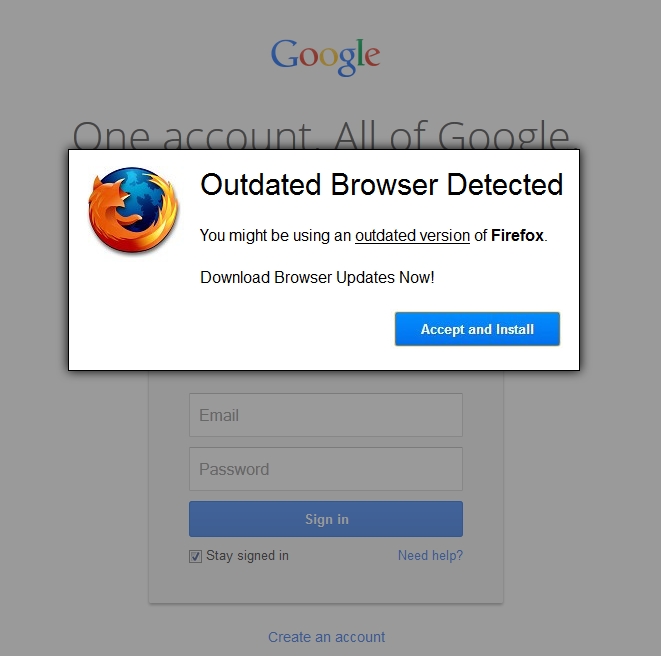
\includegraphics[width=1.0\textwidth]{ff2.png}
    \caption{This figure shows a phishing page which is prompting the user to update their browser by clicking on the link.}
   \label{fig:fakeprompt-1}
\end{figure}
\begin{figure}[p]
\centering
    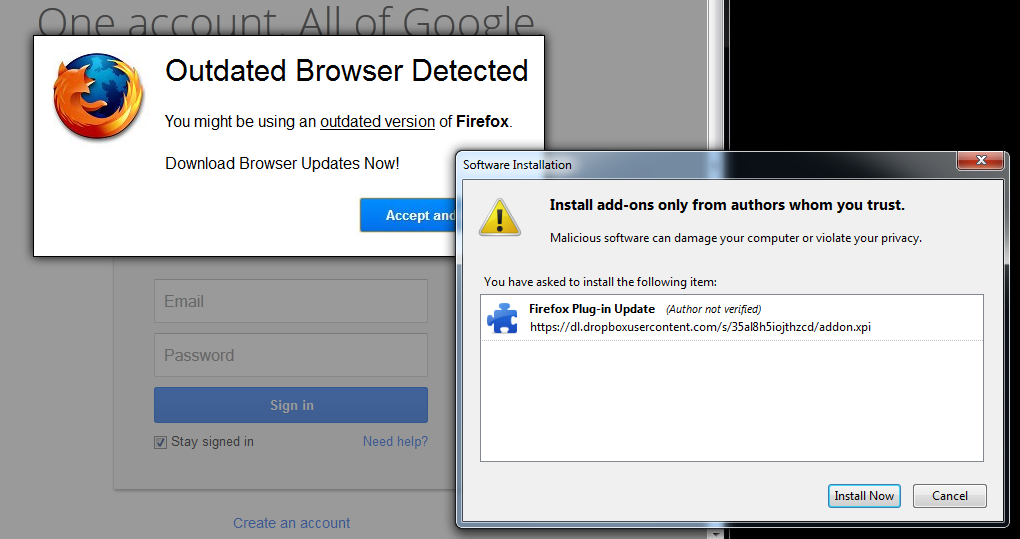
\includegraphics[width=1.0\textwidth]{ff-addon1.png}
    \caption{This figure shows the same phishing page as before after the user clicks on the link. The links leads to the browser installing a malicious add-on disguised as a fake update.}
   \label{fig:fakeprompt-2}
\end{figure}

This is made possible largely due to the use of stacking window managers in modern day systems. A stacking window manager lets the user resize, move and arrange windows in any way they want. This leads to ambiguity between which window belongs to the website and which window belongs to the system.

Figures \ref{fig:fakeprompt-1} and \ref{fig:fakeprompt-2} show an example of a phishing page which tricks the user into believing that Firefox is need of an update. When the user clicks on the update link, the browser downloads a malicious add-on. The add-on is disguised to appear as a Firefox update.

The user interface for the secure workstation must be free of such disambiguities. Taking inspiration from user interfaces of smart phones, we propose the user interface to be a single application window manager. Only one website can be displayed on the screen at any time. This is in contrast to how stacking window managers work with multiple applications overlapping each other. A single application interface will only display one application which occupies the entire screen space. In addition, there should be some screen space reserved for system prompts and notifications. Applications shouldn't be able to modify and display anything in this reserved space. Vice-versa, system prompts and notifications should never appear in the application area. This will make sure if a user sees anything in the reserved area they can trust that it is shown by the system and not by some application pretending to be the system.

Additionally, the user interface must also display the site-aggregate name and the URL of the current webpage at all times. This information should be visible in the reserved area and not writable by the websites themselves. Apart from the site-aggregate name, the user interface can also display the name of the organization or website to the user. This information can be obtained from the SSL/TLS certificates of the website.

The user may choose to mark specific websites as known and trusted. For example, the user may visit their banking website and mark it as trusted. The user interface must show visual indication whenever the user visits a trusted website. This will be helpful in case a phishing website is able to display the bank login page. The user can verify that the phishing webpage is not trusted since it does not have a trusted visual indication.

\chapter{Implementation} \label{chap:implementation}

\section{Overview}

This chapter presents the implementation of \namesecureworkstation/, a secure workstation. We use Qubes OS, an existing system described previously, as the base of our implementation. Qubes OS uses virtualization to provide the ability to run isolated applications. The implementation uses separate browser instances for each site-aggregate. Each browser instance runs in a different virtual machine providing isolation among different site-aggregates, which is the idea behind Site Aggregate Isolation policy.

Traffic from each browser instance is routed through an intermediate proxy virtual machine. This proxy VM implements a HTTP/HTTPS filter using a man-in-the-middle proxy server called {\tt mitmproxy}. The proxy server filters requests from each browser instance to enforce the other policies presented previously. To support these policies, Quboid requires additional information from the websites about their site-aggregate names, external resource requirements, etc. that it obtains from HTTP response headers.

\afterpage{\clearpage
\begin{figure}[p]
\centering
    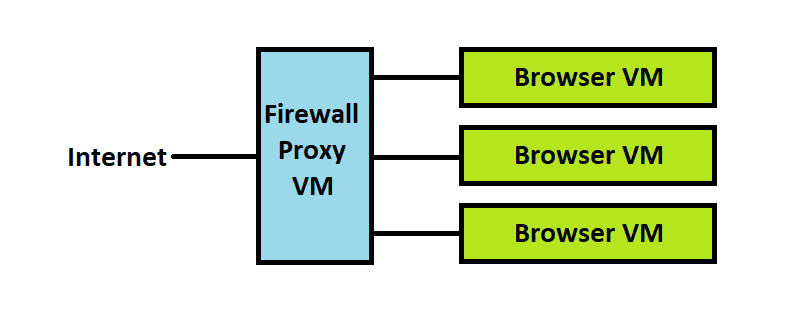
\includegraphics[width=1.0\textwidth]{design_overview.png}
    \caption{Isolation among different site-aggregates in enforced by using a separate browser instance per site-aggregate. Traffic from different browser instances is routed through an intermediate proxy virtual machine. The proxy VM runs a HTTP/HTTPS filter to filter requests from the browsers to provide isolation and enforce policies presented in this paper.}
   \label{fig:wannacry}
\end{figure}
\clearpage}

Finally, the workstation's user interface is implemented in the form of a single-application window manager. Each browser instance is displayed full-screen with no overlapping content with browser instances belonging to other site-aggregates. The interface also consists of a reserved area which is dedicated to displaying the site-aggregate of the active browser instance as well as any other system prompts. This ensures a strict separation between system content and website content.

\section{Isolation using Qubes OS}

We chose to use Qubes OS as the base for our system because of the strong isolation guarantees it provides among the different virtual machines. Browser instances are opened in separate isolated VMs and are limited to showing web pages from the same site-aggregate. Even if attacks are to exploit a browser bug to compromise the virtual machine the browser is running in, the damage is limited to the webpages from the same site-aggregate as the original website. The attack can not steal any information from other virtual machines. 

We use Firefox web browser to open webpages. The browser is configured to minimize communication with websites other than the website the user is visiting. To increase usability, a Quboid secure workstation plugin is installed in the browser. This plugin also assists the system by providing seamless switching and creation of new browser instances in case the user navigates to a webpage of a different site-aggregate. The plugin adds an additional option to open a link into a new VM when the user opens the context menu by right-clicking on the link.

The browser instances are opened in Qubes disposable VMs (DispVM). A new DispVM is created based on a preexisting template. The root filesystem of such a VM is ephemeral. Once the browser instance is closed, all changes are rolled back and the DispVM is destroyed. Thus, each browser instance is opened using a fresh image of the template runs in isolation of all other instances. This is helpful in the scenario that if one of the disposable VMs gets compromised, the damage is limited to that VM. All the state associated with that VM is destroyed as soon it is shut down.

\subsection{Other Approaches}

\paragraph{Xen Project:} Out first attempt at providing isolation was to implement a custom solution on top of Xen, a popular Linux-based hypervisor. However we soon realized the difficulty of running small lightweight virtual machines and the lack of a graphical user interface. Vanilla Xen is well-suited for running generic virtual machines in a server based settings. However, the system we envisioned was intended to be used as a workstation running applications running in lightweight virtual machines. Without a lot of modifications, it would have been impossible to achieve these goals in Xen by itself. Qubes OS on the other hand uses Xen as its base hypervisor and presents a workstation-like environment which proved ideal for our use case.

\paragraph{Custom Hypervisor:} Another approach we could have tried was to write a hypervisor customized for our needs. However, the cost of implementing a new bug-free hypervisor which can satisfy all our needs was prohibitive. Additionally, solutions such as Qubes OS and Xen have been around for a while and are well-maintained. They have been audited several times for bugs in their implementation. For a custom hypervisor to remain bug-free, its implementation would either have to be too simple to satisfy our needs or would require several hours of auditing which would have been difficult. A plausible alternative could be to write a machine-verifiable hypervisor customized for our needs. Such a hypervisor could have machine-checkable proof that it satisfies a relatively simple specification and provide a strong guarantee of being free of bugs. This approach remains unexplored.

\paragraph{Google Chrome Browser:} Google Chrome, a popular web browser, approaches the isolation problem by running its tabs in a sandboxed environment. Access restrictions are applied to a tab's rendering engine. The engine draws into an off-screen bitmap which is then presented to the user by the browser process. Each tab runs in a separate process in its own sandbox. This approach provides much of the guarantees that Qubes provides in terms of isolation. However, the problem it doesn't solve is controlled execution of untrusted files. If the user downloads a malicious file and executes it, the file will not be executed inside the sandbox. Using Qubes OS to execute untrusted files in an isolated VM solves this problem.

\section{Proxy Filter VM}

The browser virtual machines don't enforce any policies by themselves. Instead all internet traffic is routed through an intermediate proxy virtual machine. This VM enforces all the filter rules such as Site Aggregate Isolation, etc. It allows only HTTP and HTTPS traffic through. It analyzes the HTTP headers in the responses and restricts access to URLs and resources that are disallowed by any of the policies.

HTTPS connections are usually end-to-end encrypted. That means, by default the proxy VM shouldn't be able to view the contents of the request and response. To overcome this limitation, the proxy VM acts as the man-in-the-middle server between the actual target and the user. The proxy VM decrypts and re-encrypts the traffic in order to analyze and enforce the filter policies. It uses a software called mitmproxy, a web proxy written in Python.

mitmproxy generates a custom CA certificate which is then installed in the browsers as a trusted CA. Any websites that the browsers access through mitmproxy appear to be signed with a self-signed certificate by the custom CA. The mitmproxy is responsible for verifying and enforcing SSL/TLS security and inspecting the actual server certificates for validity and expiration, since this can no longer be enforced by the browsers themselves.

In order to enforce Site Aggregate policy, the proxy must obtain additional information from the website. This information includes the site-aggregate name of the website, the list of external resources needed, the allowed site-aggregates with whom the website is allowed to communicate, etc. This information is contained in the form of new HTTP response headers.

The site-aggregate name is received from the {\tt Site-Aggregate} header field. The site-aggregate name must be web-requestable URLs. The proxy must verify the name by sending a request to the site-aggregate name and checking that the requested page is in the same site-aggregate.
List of allowed URLs should be checked against the {\tt Site-Aggregate-Pattern} header field. List of allowed resources and exit destinations should be checked against the {\tt Cross-Site-Aggregate-Resource-Pattern} and {\tt Exit-Pattern} header fields.

\subsection{Other Approaches}

As opposed to redirecting the traffic through a proxy, it is also possible to enforce the policy rules in the browser itself. We decided against that approach for the following reason - in the event that a browser VM is compromised, it will leave the network exposed. The compromised VM would then be able to display and request any external resources from the internet including those belonging to different site-aggregates. There are several attacks known to exploit bugs in browser systems such as Adobe Flash or the Javascript engine. Therefore, we decided to move the enforcement away from the browser and into a separate proxy VM.

\section{Site Aggregate Isolation}

The proxy VM has the ability to inspect all traffic going between the users and web servers. The enforcement of the Site Aggregate Isolation policy is achieved by using HTTP headers. The responses from the web server contain information about its site-aggregate name, allowed exit destinations, list of external resources, etc. The proxy VM maintains a list of all the information contained the headers for each virtual machine and uses it to make decisions on whether to allow a request to go through or not.

The following subsections list the introduced HTTP headers and the policies that are used to allow or deny requests using those headers.

\subsection{HTTP Request Headers}

We do not introduce any new HTTP request headers. However, we do require the usage of the existing HTTP Referer Header \cite{rfc-referrer} \cite{mozdev-referrer}.

\paragraph{\texttt{Referer}} The {\tt Referer} header contains the URL of the previous webpage from which a link was followed. This can be used to by webpages to log the URLs from which link back to a webpage. We require the usage of this field on all requests for the purposes of filtering. Web servers must check this header field on all requests and deny any requests for which the {\tt Referer} field is not recognized. This should be enforced specifically for all the internal links of a website. If a webpage is only meant to be accessible by following internal links, access to that webpage should be prohibited from outside sources.

An example of an attack that this might prevent is when a website has a internal API which has been made public by accident. Other websites may be able to take advantage of this by listing that internet API address as an external resource and hence be able to extract information from the API.

\subsection{Resource Integrity Checks}

Several websites use CDN's to deliver scripts or stylesheets. One method to ensure that these external resources have not been tampered with to verify their integrity when they are loaded. In order to support this, a new \texttt{integrity} attribute is included for external scripts and stylesheets. The value of this attribute contains the hashed checksum of the resource to be loaded. The browser can then verify the integrity of this external resource. This method is known as Subresource Integrity \cite{subresource-integrity} \cite{subresource-integrity-2} check, and is already part of a W3C recommendation.

We encourage the use of this attribute on all static external resources to prevent malicious content to be loaded into the webpage.

\subsection{Other Approaches}

The higher level idea behind using HTTP response headers is that of providing additional information about the webpage to the secure workstation. It is possible that this information may be provided in other ways, for example, the website may have an API that provides this information. There was no compelling reason behind usage of HTTP headers as opposed to these other approaches.

It should be ensured when extracting this information that the source of the information is tamper-proof. Malicious external content must not be able to modify this information about the website. Unless the actual webserver is compromised, the source of the information must be kept isolated from the webpage content itself.

\section{Single Application Window Manager}

The final subsystem in the implementation is the user interface. The UI is a single application window manager i.e. it is designed to show exclusively display a single application at a time. This design is inspired by the user interface of smartphones, that only displays one application on the screen at a time. That advantage of this property is that the user is always aware which application is currently being displayed in the foreground. On the other side, it reduces the usability of the system since the user can no longer work on more than one application at the same time. We consider this a reasonable trade-off to create a secure and unambiguous UI.

At all times, there is a reserved area on the screen. This area is used exclusively for system UI elements. The reserved area displays the site-aggregate name of the active browser instance and any prompts by the system. Separation of the display area into a system-only area and an application-only area reduces the risk posed by phishing attacks that appear as system UI.

\begin{figure}[p]
\centering
    \fbox{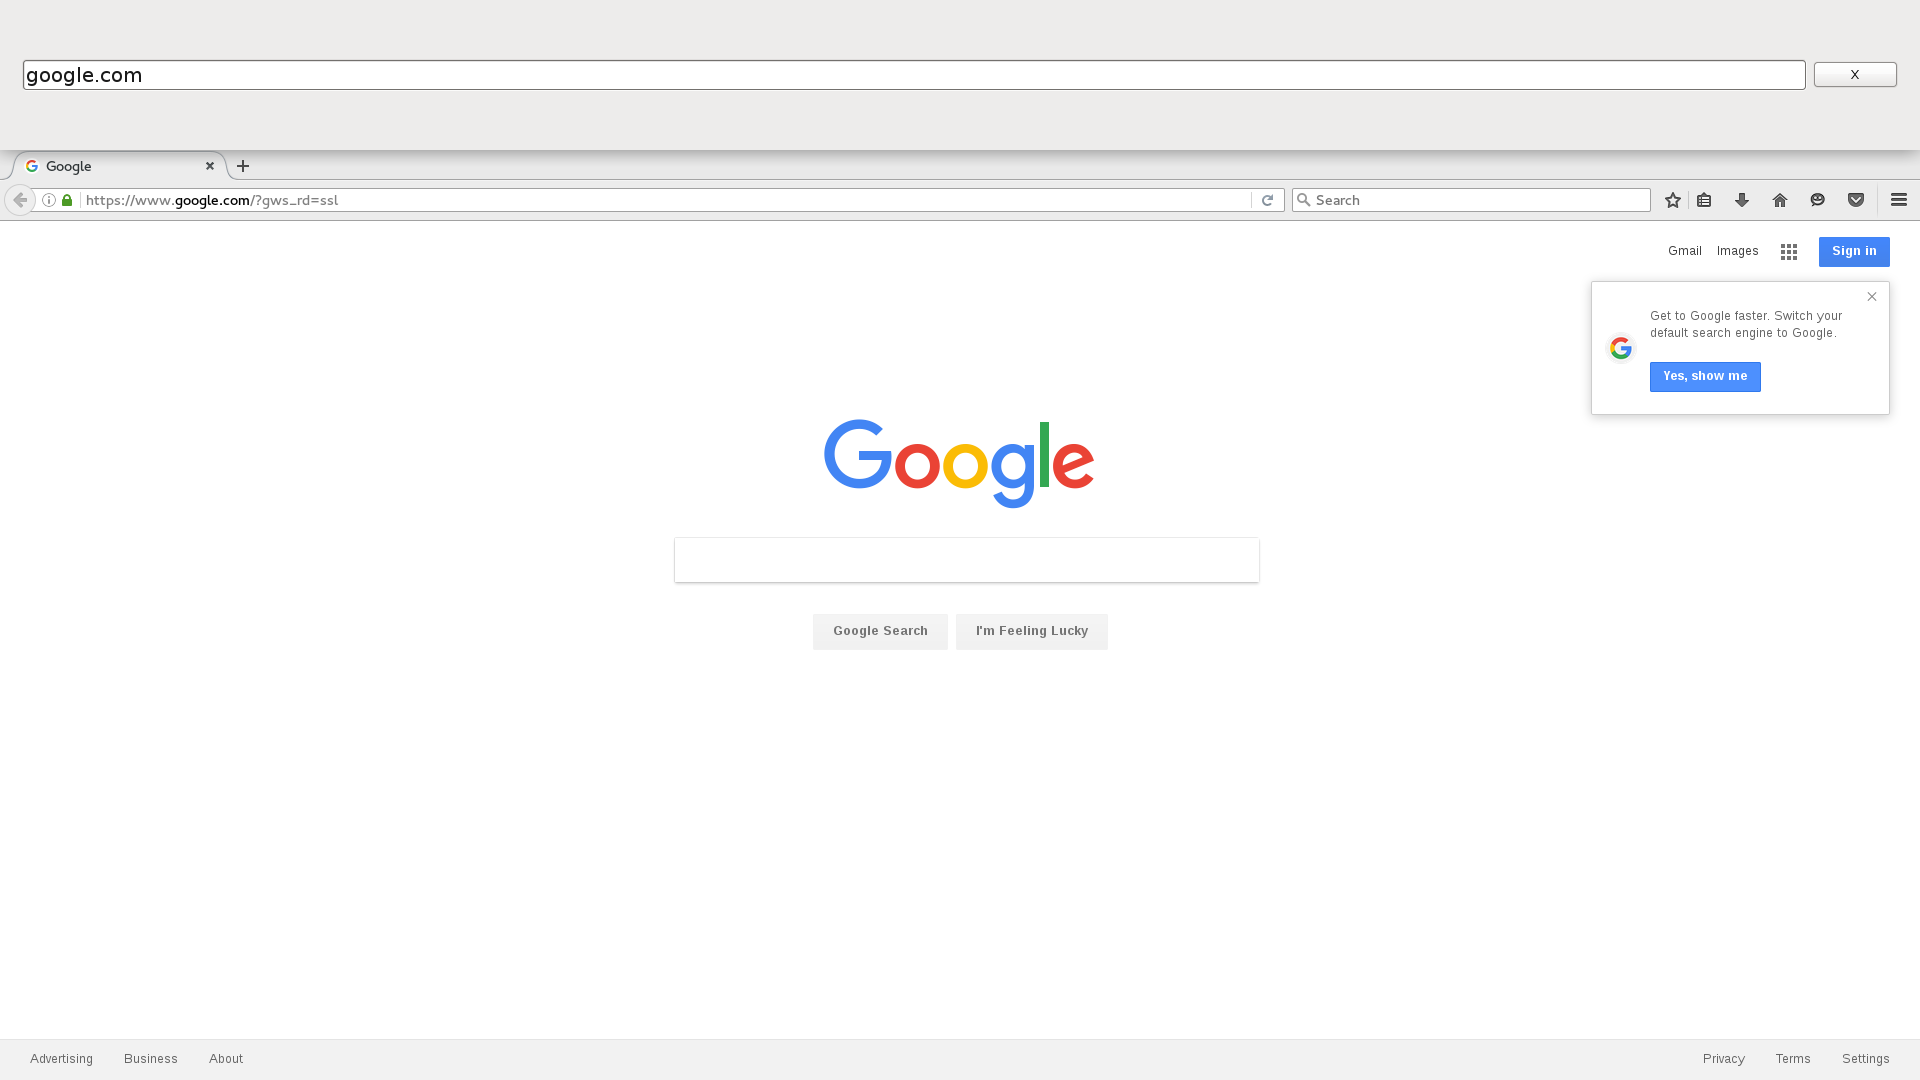
\includegraphics[width=1.0\textwidth]{ui-example.png}}
    \caption{A screenshot of the user interface of the secure workstation implementation. The top bar is a reserved area for the site-aggregate name of the active browser instance and any system prompts. The rest of the screen is used exclusively by a single browser instance.}
   \label{fig:ui-example}
\end{figure}

Figure \ref{fig:ui-example} shows a screenshot of the UI. The top reserved area permanently displays the site-aggregate name of the page visited. The user the ability to open new browser instances by typing in the site-aggregate name of the new website into the top bar.

% \section{Performance}

% We ran dd if=/dev/urandom of=test.html count=100K bs=1 and then downloaded the file
% Download 100k
% On VM:
% 876ms
% 858ms
% 862ms
% 860ms
% 858ms
% 853ms

% Direct:
% 13ms
% 18ms
% 15ms
% 12ms
% 15ms
% 17ms

% With Test server in the proxy also:
% 40ms
% 24ms
% 26ms
% 26ms
% 33ms
% 21ms


% New dispvm opening times
% 2VMs alreadybrunning
% 3.309
% 3.234
% 3.679
% 2.753
% 3.313
% 3.111

% 3VMS
% 5.044
% 5.264
% 3.276
% 3.337
% 23.244
% 3.180
% 3.790
% 3.723

% 4
% 39.874
% 4.652
% 3.113
% 4.210
% 3.711
% 3.620
% 3.402
% 3.605
% 3.312

% 5
% 4.549
% 3.942
% 4.751
% 4.747
% 5.008
% 3.371
% 3.526
% 3.241
% 3.450
% 4.364

% 6
% 4.643
% 4.589
% 4.705
% 5.307
% 4.507

% 4.540

% 4.607

% 4.843

% ~> 10
\chapter{Analysis} \label{chap:analysis}

\section{Common Attack Scenarios}

Here is a list of common phishing attacks and how \namesecureworkstation/ defends against such attacks.

\subsection{Attacks via email}

\paragraph{Scenario:} The first attack is a popular phishing email attack \cite{attack-verify-email}. The user receives an email appearing to come from Microsoft. It claims that unless the user ``verifies" their account, their account may be closed down. The link to verify leads to a fake sign in page tricking the users to enter their credentials. Figure \ref{fig:attack-verify-email} shows an example of such a phishing email.

\paragraph{Currently:} If the user overlooks the source of the email address (which is onmicrosoft.com) and the URL of the fake sign in page, their credentials will be stolen by the attacker.

\paragraph{Quboid:} Clicking on the verify link opens up a new browser instance with an unrecognized domain name. The interface warns the users that this page has an unrecognized domain. The top area also displays the site-aggregate name of the web page not being Microsoft. The user looks at these cues and recognizes that the web page is a phishing page. However, if the user does not recognize these cues, their credentials may still get stolen by the attacker.

\afterpage{\clearpage}
\begin{figure}[p]
\centering
    \fbox{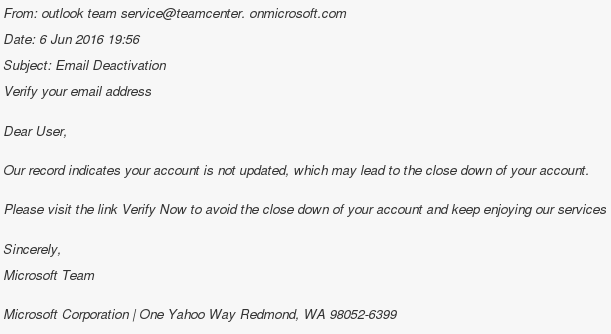
\includegraphics[width=1.0\textwidth]{attack-verify-email.png}}
    \caption{This phishing email appears to come from Microsoft but the domain is suspicious (onmicrosoft.com). The verify link contained in the email leads the user to a fake login page.}
   \label{fig:attack-verify-email}
\end{figure}

\paragraph{Similar Attacks:} There are several other attacks that work in similar ways as to this attack \cite{attack-verify-email-1}\cite{attack-verify-email-2}\cite{attack-verify-email-3}. All these emails start out with a threat of having the user's account closed and asks the user to enter their credentials on a fake login page.

\noindent\rule[0.5ex]{\linewidth}{1pt}

\paragraph{Scenario:} A majority of phishing emails aim at delivering ransomwares to the users. A report by PhishMe estimates that over 97\% of phishing emails deliver ransomwares. The user receives an email asking them to open an attachment which contains information of a delivery as a ZIP file. The attachment contains a ransomware executable. Figure~\ref{fig:attack-ransomware} shows an example of such an email.

\paragraph{Currently:} Upon opening, the ransomware starts executing and encrypts the user's hard disk.

\paragraph{Quboid:} The attachment opens in a new isolated virtual machine since the link belonged to a different site-aggregate. Even though the ransomware is able to execute, it does no damage since it can access only the contents of the isolated virtual machine. It also doesn't have access to data from other browser instances since they run in separate virtual machines. This prevents the malicious software to steal data associated with logged in sessions on other websites.

\begin{figure}[p]
\centering
    \fbox{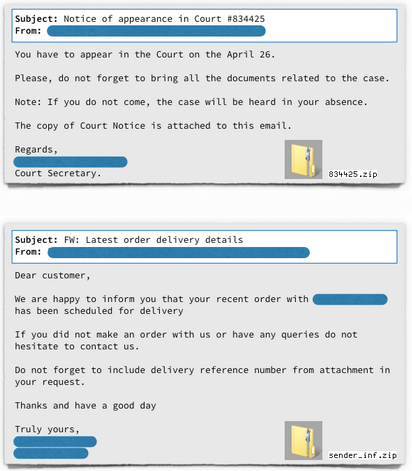
\includegraphics[width=1.0\textwidth]{attack-ransomware-email.png}}
    \caption{This phishing email appears to contain legitimate content but instead contains a ransomware in the attached ZIP file.}
   \label{fig:attack-ransomware}
\end{figure}

\paragraph{Similar Attacks:} A variant of this attack is a phishing email which doesn't actually has any attachment but has an image which appears to be an attachment. To an unsuspecting user, it appears to be a legitimate attachment and he/she expects that the attachment has already been scanned for malware by the email client. However, the attachment image is actually a link that redirects to a page that downloads the malware.

\subsection{Malvertisements}

Malvertisements is another way in which phishing attacks can occur. The internet economy is based on online advertisements. Large websites offer ad spaces by directly contacting target companies. Small scale websites, on the other hand, use intermediate advertising services in order to display ads. If one of these intermediate services gets compromised, all other websites that use that service may get compromised as well. Specifically, consider the following scenario:

\paragraph{Scenario:} The user is browsing a website which uses an external advertisement provider. The provider's system was compromised and the attacker has uploaded a malicious advertisement. For example, if a bank website is displaying an advertisement, the advertisement might claim to be a credit card sign-up form and ask the user for their social security number.

\paragraph{Currently:} The user thinks that it is a genuine form and submits their details to the attacker's server. The attacker can then steal the information entered in the form.

\paragraph{Quboid:} Although the user might enter their details into the fake form, since the bank website does not list the attacker's server as an allowed exit destination, the browser is forbidden from communicating any information to the server. Clicking on the link will just open a new browser instance with the submit URL of the form without any form data being submitted along with the request. This mechanism only works if the external advertisement does not include malicious Javascript. For example, most email client block any Javascript from executing in HTML emails. A malicious script may be able to encode the form data in other ways, thus defeating the purpose of controlling the exit URLs.

\paragraph{Similar Attacks:} Similarly, the advertisement can display a link to fake login page. However, if that link belongs to a different site-aggregate, the URL will open in a separate browser instance and the interface will clearly show the site-aggregate name of the new web page.

\subsection{Attacks using User Interface Ambiguity}

\paragraph{Scenario:} While visiting a website, a popup appears which looks like the Chrome prompt. The prompt says that the user's computer is infected with a virus and an antivirus software must be downloaded. The software downloaded is actually a malware.

\paragraph{Currently:} The popup appears indistinguishable from the actual system prompt to an unsuspecting user. The user downloads the infected software.

\paragraph{Quboid:} The user expects system prompts to be displayed only in the reserved area. Hence, there is a higher chance of the user suspecting something is wrong if any system-prompt looking content is displayed in the application content area.

% \noindent\rule[0.5ex]{\linewidth}{1pt}

% \paragraph{Scenario:} You get an email saying you need to ``verify" your account, else it will be deactivated. There is a link in the email that points to a webpage which asks you to enter your password.

% \paragraph{Currently:} You get an email saying you need to ``verify" your account, else it will be deactivated. There is a link in the email that points to a webpage which asks you to enter your password.

% \paragraph{Solution:} You get an email saying you need to ``verify" your account, else it will be deactivated. There is a link in the email that points to a webpage which asks you to enter your password.

% \noindent\rule[0.5ex]{\linewidth}{1pt}

% \paragraph{Scenario:} You get an email saying you need to ``verify" your account, else it will be deactivated. There is a link in the email that points to a webpage which asks you to enter your password.

% \paragraph{Currently:} You get an email saying you need to ``verify" your account, else it will be deactivated. There is a link in the email that points to a webpage which asks you to enter your password.

% \paragraph{Solution:} You get an email saying you need to ``verify" your account, else it will be deactivated. There is a link in the email that points to a webpage which asks you to enter your password.

% \noindent\rule[0.5ex]{\linewidth}{1pt}

% \paragraph{Scenario:} You get an email saying you need to ``verify" your account, else it will be deactivated. There is a link in the email that points to a webpage which asks you to enter your password.

% \paragraph{Currently:} You get an email saying you need to ``verify" your account, else it will be deactivated. There is a link in the email that points to a webpage which asks you to enter your password.

% \paragraph{Solution:} You get an email saying you need to ``verify" your account, else it will be deactivated. There is a link in the email that points to a webpage which asks you to enter your password.

% \noindent\rule[0.5ex]{\linewidth}{1pt}

% \paragraph{Scenario:} You get an email saying you need to ``verify" your account, else it will be deactivated. There is a link in the email that points to a webpage which asks you to enter your password.

% \paragraph{Currently:} You get an email saying you need to ``verify" your account, else it will be deactivated. There is a link in the email that points to a webpage which asks you to enter your password.

% \paragraph{Solution:} You get an email saying you need to ``verify" your account, else it will be deactivated. There is a link in the email that points to a webpage which asks you to enter your password.

% \noindent\rule[0.5ex]{\linewidth}{1pt}

\subsection{Other Attacks}

\paragraph{Scenario:} An attacker is able to poison the DNS resolver cache of the user's local system. The new entries point to the attackers server where a fake login page is displayed.

\paragraph{Currently:} The user believes the fake login page to be genuine and enters their credentials. The attacker can not steal these credentials.

\paragraph{Quboid:} Since the DNS resolver cache is poisoned, it fails DNSSEC integrity checks. The proxy VM blocks the request from going through in the first place.

\noindent\rule[0.5ex]{\linewidth}{1pt}

\paragraph{Scenario:} An attacker may be using a man-in-the-middle server to sniff all the content that the user is browsing. In the usual case, any traffic that has been encrypted using SSL/TLS should not be visible to the attacker. However, if the attacker is able to obtain a fake certificate for a website which was issued by a trusted CA, the man-in-the-middle server may be able to sniff the encrypted traffic to that website as well.

\paragraph{Currently:} If the fake certificate was issued by a trusted CA, there is no way the user can identify that such an attack is taking place.

\paragraph{Quboid:} The DNS records for the website also contains DANE entries. These entries have the public the key of the certificate that the website uses. Since the keys in the DNS record and the keys in the certificate presented by the attacker will not match up, the system will reject the request and notify the user that the DANE validation failed.

% \begin{itemize}
%     \item  You get an email saying you need to “verify” your account otherwise it will be deactivated. The link goes to a link that asks for your password.

%     \item Poisoning DNS caches to redirect common websites to attackers versions.

%     \item Lured victims into entering their dropbox credentials on a page hosted on dropbox itself. Similarly, for any other websites which let you host content. http://www.csoonline.com/article/2953190/vulnerabilities/google-drive-phishing-is-back-with-obfuscation.html http://www.symantec.com/connect/blogs/dropbox-users-targeted-phishing-scam-hosted-dropbox

%     \item Email stating someone sent you a Google Doc. You open it, and it leads to a OAuth authorization page stating the app needs access. You click yes, the page redirects to an external attackers link with an authorized token.

%     \item RSA security keys were stolen when a flash vulnerability was used in a spear phishing attack.

%     \item Nigerian Prince scam wire money to this account/dating website email

%     \item Malicious Email with a malicious email attachment.

%     \item Placed phishing content on a legitimate server of some org. E.g. paypal login on srilankan government page

%     \item Go to a website, popup comes says download a software in order to access something. It is a malicious software

%     \item Popup comes saying you have a problem with your computer, call number to connect to a tech support service.

%     \item We have recieved a password reset request, please go to this webpage and enter your old password.

%     \item A post on a legitimate website e.g. Airbnb requesting to circumvent the website’s payment procedure and use an external service e.g. western union. You may get an email saying the same with a scam email address.

%     \item Fake online surveys which may ask for personal information

%     \item Tracking notification for UPS containing a malicious exe

%     \item Online websites which send you fake goods

%     \item Facebook fake friend

%     \item Tax services scams

%     \item Credentials stolen on Steam. Attackers can put arbitrary javascript code in their profile. Can be used to redirect users to some other page, steal login cookie.

%     \item Link is a data:text/html url containing a whole login page. The link is disguised as an attachment.

%     \item Lastpass users tricked into entering their credentials on a fake lastpass page.

%     \item Puny code lets you get https certs for a fake domain which appears as real domain on your browser

%     \item M.facebook.com---------------------------------.stuff

%     \item Blockhain.com

%     \item Search engine phishing/credit card offers - give up personally identifiable information

%     \item Sometimes legit sites don’t include ownership information in their SSL certificates. Additionally they may use multiple domains. Impossible to identify right from wrong. Either verify the website externally, or SRP like password.

%     \item LetsEncrypt makes Chrome show “Secure” on the URL bar. Anyone can create certs.
% \end{itemize}

\subsection{Attacks that Quboid does not defend against}

Quboid provides several mechanism to make the user aware that a phishing attack may be taking place. However, it is still possible for the user to overlook these cues. In these cases, Quboid does not prevent against the effects resulting from these attacks.

\paragraph{Scenario:} The user unknowingly visits a malicious site which has a pop-up notifying that their computer may have a virus and they need to call the given phone number in order to request tech support. If the user fails to notice that this prompt was not generated by the system, they continue with the call and may potentially reveal sensitive information. Since this is a completely offline attack, our system cannot defend against this attack.

\paragraph{Scenario:} If the user fails to notice the site-aggregate name of a website being displayed in the top reserved area, it is possible for a phishing attack to still succeed by displaying fake login pages. Although Quboid provide several cues, an uncareful user may be able to miss them.

\section{Quboid Defense Mechanisms}

Quboid employs several defense mechanisms as we saw in earlier chapters. Here we list these defense mechanisms and explain the attack scenarios that they prevent:

\paragraph{Separate VM's:} Each browser instance runs in a separate VM. In the event that the user executes a malicious downloaded file, the damage remains contained within that virtual machine.

\paragraph{Site Aggregates:} Websites forming a single unit are grouped together in a single site-aggregate. Phishing websites which pretend to be other website will not be part of this aggregate and Quboid will display this information.

\paragraph{Proxy Filter:} All network traffic is routed through an intermediate proxy. The proxy ensures that a virtual machine can access content only from its own site-aggregate, even in the event that the virtual machine has itself been compromised.

\paragraph{Exit URL Whitelist:} A whitelist is contained in the HTTP response headers which lists the URLs that a page is allowed to submit form data to. This is helpful in case the browser displays external HTML-only content where the external content has been compromised. It prevents data being submitted outside of the site-aggregate of the browser.

\paragraph{External Resources Whitelist:} The external resources whitelist allows sites to retrieve content from external websites but prevents the browsers from navigating directly to these websites.

\paragraph{Secure User Interface:} The user interface of Quboid is separated into two: application and system. This prevents attacks where a website may try to fake a system prompt and lead the user into downloading malicious software.

\section{Implementation Overhead}

\subsection{Network Latency}

All network traffic is routed through a proxy VM. This results in an increased latency during web browsing. We measured this latency by first measuring the latency when requesting a web page without going through a proxy, and then measuring the latency with the proxy. We used \texttt{mitmproxy}, a Python based proxy, for our measurements and implementation.

Figure~\ref{fig:latency} lists the average latency measured in three different scenarios: (1) without a proxy VM, (2) through a proxy without any filter rules, and (3) through a proxy with filter rules.

\begin{figure}
\centering
    \begin{tabular}{| l | l |}
    \hline
    \textbf{Scenario} & \textbf{Latency} \\ \hline
    Without proxy & 15ms $\pm$ 2ms \\ \hline
    With proxy without filter & 28ms $\pm$ 6ms \\ \hline
    With filter proxy & 860ms $\pm$ 7ms \\ \hline
    \hline
    \end{tabular}
\caption{Average latency in different proxy configurations} \label{fig:latency}
\end{figure}

We find that the latency introduced just by adding an intermediate proxy is not significant. However, filter rules adds significant amount of latency. This latency can be reduced by having more efficient implementations of the proxy software and of the filter.

\subsection{Virtualization Overhead}

Although Qubes employs various techniques to speed up virtual machine creation, it still takes some time to start new VMs. We measured the time it takes to open new browser instances in Qubes disposable VMs. We measured the opening times with different number of virtual machines already running on the system. This shows any performance limitations that could arise during the normal browsing experience.

Figure~\ref{fig:openvm} shows a plot of the average time to open new VMs vs. number of existing running VMs. We imagine that in a normal browsing session, the user has around 6-7 web-aggregates open in the VMs. For up to that number of VMs, we do not see any significant performance hit.

$ $\\

\begin{figure}
\centering
\begin{tikzpicture}[y=1cm, x=1cm,font=\sffamily]
 	%axis
	\draw (0,0) -- coordinate (x axis mid) (7,0);
    	\draw (0,0) -- coordinate (y axis mid) (0,6);
    	%ticks
    	\foreach \x in {0,...,7}
     		\draw (\x,1pt) -- (\x,-3pt)
			node[anchor=north] {\x};
    	\foreach \y in {0,...,6}
     		\draw (1pt,\y) -- (-3pt,\y) 
     			node[anchor=east] {\y}; 
	%labels      
	\node[below=0.8cm] at (x axis mid) {\# of existing VMs};
	\node[rotate=90, above=0.8cm] at (y axis mid) {Time to open new VM [s]};

	%plots
	\draw plot[mark=square*]
		file {openvm.data};  
\end{tikzpicture}
\caption{Plot of average VM opening time vs. the number of existing running VMs} \label{fig:openvm}
\end{figure}

\subsection{User Experience}

Quboid changes the browsing experience for the user in a number of ways.

\paragraph{Separate VMs per site-aggregate:} Each site-aggregate is opened in a separate VM. Opening new VMs is slower than opening new tabs in a modern web browser. This is a trade-off that Quboid makes between usability vs. the security offered by virtualization.

\paragraph{Single Application Window Manager:} Quboid diverges from the more popular tiling window managers by using a single application window manager. Only one browser instance may be displayed on the screen at a time. Different browser instances are switched by using the application switching shortcuts in the window manager. This restricts the usability in the event that the user needs to look at content from multiple browser instances at the same time.

\paragraph{Restricting downloads to VMs:} Any application downloaded by the user is run in a separate VM. Thus, it cannot access content from applications running in different VMs. Everyday tasks such as downloading a media player to play movies require extra steps since the user has to now move the movie to the media player VM before playing.

\chapter{Conclusion} \label{chap:conclusion}

Phishing attacks are a source of several major cyberattacks. As recent attacks have demonstrated, current systems are insufficient to prevent these attacks. This thesis presented the design an implementation of a workstation to help defend against phishing attacks.

This thesis introduced policies which are focused to minimize the risk of phishing attacks. The policy of Site Aggregate Isolation dictated that websites which are of different site-aggregates must not share any state with each other and must not be able to communicate with each other. In view of modern web applications, we introduced exceptions to this policy to support loading resources from other site-aggregates. Lastly, we outlined the design of an unambiguous user interface that clearly identifies the source of any content displayed on the screen.

We developed \namesecureworkstation/, a system based on Qubes OS to provide isolated browser instances belonging to different site-aggregates running in different virtual machines. The system consists of a transparent web proxy which filters the traffic based on the previously mentioned policies. We introduced new HTTP response headers to provide additional information about the web pages in order to support filtering in the proxy. We also implemented a user interface with reserved areas to display system and application content, and a clear display of the site-aggregate name of the active browser instance.

We analyzed the effectiveness of the design by looking at recent phishing attacks and fictional scenarios. We played out how users would react using current systems in these scenarios and how would our design help defend against these attacks.

Quboid is a system which helps the user in identifying phishing attempts. However, the system does have limitations. It does not prevent phishing attacks completely but reduces the likelihood of a successful attack. If users miss the cues provided by the system, they are still vulnerable to these attacks.

\section{Future Work}

The work performed in this thesis exclusively focused on defense against phishing attacks. We approached the design of \namesecureworkstation/ by reviewing recent phishing attacks and fictional scenarios. But if we take a step back, the reason behind phishing attacks is the ambiguity of authorship in modern internet. There was a time when visiting some website meant all the content the user sees is authored exclusively by the website owner. SSL/TLS certificates were invented which further strengthen the user's belief that the website they are is legitimate and has been externally vetted by trusted certificate authorities. However, with time both of these trends seem to have changed.

Websites like Facebook and Reddit contain majority of content which has not been authored by the website owners but rather by the visitors of the website. Several certificate authorities have been established, some that allow users to gain certificates for their websites at no cost. These authorities just verify website ownership but not if the owner is a genuine entity. The times have changed and modern internet needs are a lot of different.

In view of these changing needs, we need systems in place that can not only verify the authenticity of a website as whole but also parts of the website. We need methods to be able to verify the authorship of the content posted on the websites by other users. The failure of verification of authorship is what leads to phishing attacks.

This is a more general problem than what the system presented in this thesis solves. One can envision an internet where every part of a website carries a proof of authenticity and ownership. Then the user may be able to specify policies based solely on the authorship rather than the different parameters that we mentioned in the design of Quboid.

% \appendix
% \chapter{Tables}

\begin{table}
\caption{Armadillos}
\label{arm:table}
\begin{center}
\begin{tabular}{||l|l||}\hline
Armadillos & are \\\hline
our	   & friends \\\hline
\end{tabular}
\end{center}
\end{table}

\clearpage
\newpage

% \chapter{Figures}

\vspace*{-3in}

\begin{figure}
\vspace{2.4in}
\caption{Armadillo slaying lawyer.}
\label{arm:fig1}
\end{figure}
\clearpage
\newpage

\begin{figure}
\vspace{2.4in}
\caption{Armadillo eradicating national debt.}
\label{arm:fig2}
\end{figure}
\clearpage
\newpage

%% This defines the bibliography file (main.bib) and the bibliography style.
%% If you want to create a bibliography file by hand, change the contents of
%% this file to a `thebibliography' environment.  For more information 
%% see section 4.3 of the LaTeX manual.
% \begin{singlespace}
% \bibliography{main}
% \bibliographystyle{plain}
% \end{singlespace}

\begin{thebibliography}{99}
\begin{singlespace}
\raggedright

\bibitem{dnc-hack}
``Top Democrat's emails hacked by Russia after aide made typo, investigation finds," December 14, 2016. Available: \url{https://www.theguardian.com/us-news/2016/dec/14/dnc-hillary-clinton-emails-hacked-russia-aide-typo-investigation-finds}

\bibitem{wannacry-uk}
``UK hospitals hit with massive ransomware attack," May 12, 2017. Available: \url{https://www.theverge.com/2017/5/12/15630354/nhs-hospitals-ransomware-hack-wannacry-bitcoin/}

\bibitem{phishme-report}
``2016 Enterprise Phishing Susceptibility and Resiliency Report," 2016. Available: \url{https://phishme.com/2016-enterprise-phishing-susceptibility-report/}

\bibitem{91phishing}
``91\% Of Cyberattacks Start With A Phishing Email," December 13, 2016. Available: \url{http://www.darkreading.com/endpoint/91–of-cyberattacks-start-with-aphishing-email/d/d-id/1327704}

\bibitem{phishing-example-paypal}
``Phishing Example: PayPal - We need your help," March 22, 2016. Available: \url{https://security.berkeley.edu/news/phishing-example-paypal-we-need-your-help}

\bibitem{phishing-example-malware}
``Phishing Example: Messages containing Locky malware," August 24, 2016. Available: 
\url{https://security.berkeley.edu/news/phishing-example-messages-containing-locky-malware}

\bibitem{deep-packet-inspection}
``Firewall Evolution - Deep Packet Inspection," July 28, 2003. Available: \url{https://www.symantec.com/connect/articles/firewall-evolution-deep-packet-inspection}

\bibitem{qubes-os}
``Qubes OS: A resonably secure operating system." Available: \url{https://www.qubes-os.org/}

\bibitem{xen}
``The Xen Project, the powerful open source industry standard for virtualization." Available: \url{https://www.xenproject.org/}

\bibitem{bromium}
``Understanding Bromium\textsuperscript{\textregistered} Micro-virtualization for Security Architects." Available:
\url{https://www.bromium.com/sites/default/files/Bromium\%20Microvirtualization\%20for\%20the\%20Security\%20Architect_0.pdf}

\bibitem{marketsharereport}
``Google's Chrome Browser crushes the desktop competition in 2016," Feb 16, 2017. Available: \url{https://www.forbes.com/sites/kevinmurnane/2017/02/16/googles-chrome-browser-crushes-the-desktop-competition-in-2016/}

\bibitem{chromesandbox}
``Sandbox." Available: \url{https://chromium.googlesource.com/chromium/src/+/master/docs/design/sandbox.md}

\bibitem{google-docs-phishing}
``Google Docs users hit with sophisticated phishing attack," May 3, 2017. Available: \url{https://www.theverge.com/2017/5/3/15534768/google-docs-phishing-attack-share-this-document-with-you-spam}

\bibitem{gmail-spam-filter-list}
``Why emails are automatically marked as spam." Available: \url{https://support.google.com/mail/answer/1366858#warnings}

\bibitem{eros}
``Design of the EROS Trusted Window System." Available: \url{https://www.usenix.org/legacy/publications/library/proceedings/sec04/tech/full_papers/shapiro/shapiro.pdf}

\bibitem{fake-attachment-scam}
``Beware This Clever `Fake Attachment' Gmail Phishing Scam," Mar 15, 2017.Available: \url{https://www.lifehacker.com.au/2017/03/beware-this-clever-fake-attachment-gmail-phishing-scam/}

\bibitem{malvertising}
``What is Malvertising?" September 5, 2014. Available: \url{https://www.kaspersky.com/blog/what-is-malvertising/5928/}

\bibitem{malvertisement-nytimes}
``New York Times, BBC and others inadvertently serve up dangerous ads," March 16, 2016. Available: \url{https://www.cnet.com/news/new-york-times-bbc-dangerous-ads-ransomware-malvertising/}


\bibitem{punycode-attack}
``Chrome, Firefox and Opera vulnerable to Punycode phishing attack," April 20, 2017. Available: \url{https://www.theinquirer.net/inquirer/news/3008708/chrome-firefox-and-opera-vulnerable-to-punycode-phishing-attack}

\bibitem{chinese-ca}
``Chinese Certificate Authority `mistakenly' gave out SSL Certs for GitHub Domains,'' August 29, 2016. Available: \url{http://thehackernews.com/2016/08/github-ssl-certificate.html}

\bibitem{rfc-referrer}
``RFC 7231 - Hypertext Transfer Protocol (HTTP/1.1) - Section 5.5.2," June 2014. \url{https://tools.ietf.org/html/rfc7231#section-5.5.2}

\bibitem{mozdev-referrer}
``Referrer." \url{https://developer.mozilla.org/en-US/docs/Web/HTTP/Headers/Referer}

\bibitem{subresource-integrity}
``Subresource Integrity," June 23, 2016. Available: \url{https://www.w3.org/TR/SRI/}

\bibitem{subresource-integrity-2}
``Subresource Integrity." Available:  \url{https://developer.mozilla.org/en-US/docs/Web/Security/Subresource\_Integrity}

\bibitem{attack-verify-email}
``Beware of ``Email Deactivation - Verify Your Email Address" Microsoft Phishing Scam," June 7, 2016. Available: \url{https://www.onlinethreatalerts.com/article/2016/6/7/beware-of-email-deactivation-verify-your-email-address-microsoft-phishing-scam/}
\bibitem{attack-verify-email-1}
```Verify Your Email Account', The Latest Phishing Scam to Emerge Online," April 4, 2015. Available: \url{https://www.hackread.com/verify-your-email-account-the-latest-phishing-scam-to-emerge-online/}
\bibitem{attack-verify-email-2}
```Google email verification' message." Available: \url{https://support.google.com/accounts/answer/32044}
\bibitem{attack-verify-email-3}
``UChicago: Latest Email Scams." Available: \url{https://itservices.uchicago.edu/page/latest-email-scams}

\end{singlespace}
\end{thebibliography}
\end{document}

